% (C) Anders Kofod-Petersen
\documentclass[a4paper]{book}
\usepackage[english]{babel}						% Correct English hyphenation
%\usepackage[latin1]{inputenc}						% Allow for non-English letters
\usepackage[utf8]{inputenc}
\usepackage{graphicx}							% To include graphics
\usepackage{natbib}								% Correct citations
\usepackage{fancyheadings}						% Nice header and footer
\usepackage[linktocpage,colorlinks,pdfpagelabels]{hyperref}			% PDF hyperlink
\usepackage{geometry} 							% Better geometry
\usepackage{mathtools}                          % for typing math
\usepackage{amsmath}
%\usepackage[center]					% For cropping documents
\usepackage{rotating}
\usepackage{algorithm}
\usepackage{algorithmic}
\usepackage{float}
\usepackage{mathtools}
\usepackage{import}
\usepackage{listings}
%\graphicspath{{nn/}}
% B5 (uncomment to convert to B5 format)
 \geometry{b5paper}
\usepackage[toc,page]{appendix}
% Author
% Fill in here, and use commands in the text. 
\newcommand{\thesisAuthor}{Andreas Hagen}
\newcommand{\thesisTitle}{Evolving altruism through kin recognition in evolutionary robotics}
\newcommand{\thesisType}{Master's thesis}
\newcommand{\thesisDate}{Spring 2014}

% PDF info
\hypersetup{pdfauthor={\thesisAuthor}}
\hypersetup{pdftitle={\thesisTitle}}
\hypersetup{pdfsubject={\thesisType}}
\hypersetup{linkcolor=black}
\hypersetup{citecolor=black}
\hypersetup{urlcolor=black}

%Fancy headings
\pagestyle{fancy}
\pagestyle{fancyplain}
\renewcommand{\chaptermark}[1]{\markboth{#1}{}}
\renewcommand{\sectionmark}[1]{\markright{#1}{}}
\lhead[\fancyplain{}{\thepage}]{\fancyplain{}{\let\uppercase\relax\leftmark}}
\rhead[\fancyplain{}{\let\uppercase\relax\rightmark}]{\fancyplain{}{\thepage}}
\chead[\fancyplain{}{}]{\fancyplain{}{}}
\lfoot[\fancyplain{}{}]{\fancyplain{}{}}
\cfoot[\fancyplain{}{}]{\fancyplain{}{}}
\rfoot[\fancyplain{}{}]{\fancyplain{}{}}
% Citation format
\bibliographystyle{apalike}
\bibpunct{[}{]}{;}{a}{,}{,}

\begin{document}

%Title page (This is generate automatically from the commands above)
\begin{titlepage}
\noindent {\large \textbf{\thesisAuthor}}
\vspace{2cm}

\noindent {\Huge \thesisTitle}
\vspace{2cm}

\noindent \thesisType, \thesisDate 
\vspace{2cm}

\noindent Artificial Intelligence Group\\ Department of Computer and Information Science\\ Faculty of Information Technology, Mathematics and Electrical Engineering\\

\vfill
%\begin{figure}[p]
\begin{center}
\centering

\includegraphics[trim=12cm 10cm 13cm 14cm, scale=0.9]{ntnu.pdf}
\end{center}
%\end{figure}
\end{titlepage}

\thispagestyle{empty}

\cleardoublepage

\frontmatter

\section*{Abstract}


In this paper the different mechanisms that enable the evolution of altruistic behavior in evolutionary computation are explored. 
The research is motivated by the need for systems using embodied evolution to evolve relevant traits needed to avoid extinction in a dynamic environment.
In particular interest is the subject of self-sacrifice where individuals relinquish the chance of reproduction altogether to assist others. 
The paper contains a structured literature review on altruism in simulated environments in artificial evolution. 
The literature review results in the question of whether or not kin-selection is a prerequisite for the evolution of self-sacrifice.  

%\begin{itemize}
%\item the field of research
%\item a brief motivation for the work
%\item what the research topic is and
%\item the research approach(es) applied. 
%\item contributions
%\end{itemize}

%The abstract length should be roughly half a page of text --- without lists, tables or figures.  

\clearpage

\section*{Preface}



\vspace{1cm}

This report was written as a master's thesis in the spring of 2014 at the Norwegian University of Science and Technology. It was officially supervised by Pauline Haddow with assistance by Jean-Marc Montanier.
%The preface includes the facts - what type of project, where it is conducted, who supervised and any acknowledgements you wish to give. 

\vfill

\hfill \thesisAuthor

\hfill Trondheim, \today

\clearpage

\tableofcontents

%\listoffigures

%\listoftables

\mainmatter

\chapter{Introduction}
\label{cha:Introduction}

%This paper explores the research done on mechanisms that are responsible for the evolution of altruistic behavior and in the most extreme case; the act of self-sacrifice.
%The intended use is within the field of evolutionary computation where wanted behavior is often found by mimicking the mechanisms of natural evolution. 
%The goal of the paper is to shed light on how the mechanisms we know to exist from nature have been utilized in the artificial evolution of altruism.
%Section \ref{sec:BackgroundAndMotivation} gives a cursory introduction to the evolution of altruism and cooperation and outlines why research on altruism is of interest in artificial intelligence.
%Chapter \ref{cha:review} gives a review of the existing literature related to the mechanisms behind altruism and the simulation of these mechanisms in simulated 
%environments. Chapter \ref{cha:discussion} gives a discussion of some of the questions that arise from the literature review and proposes a research question
%that addresses one of the issues brought to attention. Some thoughts on how this question should be researched is also given. The protocol for the structured literature review and the documentation of the review is given in chapter \ref{cha:STL}

%All chapters should begin with an introduction before any sections begin. Further, each sections begins with an introduction before  subsections begin. Chapters with just one section or sections with just one sub-section, should be avoided. Think carefully about chapter and section titles as each title stand alone in the table of contents (without associated text) and should convey meaning for the contents of the chapter or section. 

%In all chapters and sections it is important to write clearly and concisely. Avoid repetitions and if needed, refer back to the original discussion or presentation. Each new section, subsection or paragraph should provide the reader with new information and be written in your own words. Avoid direct quotes. If you use direct quotes, unless the quote itself is very significant, you are conveying to the reader that you are unable to express this discussion or fact yourself. Such direct quotes also break the flow of the language (yours to someone else's).   



One main area of interest in altruism in evolutionary robotics is within the field of multi- agent systems, especially within embodied evolution where agents are continuously adapting to the environment. One of the long-term goals in this field is to create agile populations of robots that are able to create new solutions to previously unseen problems that  arise and have the necessary mechanisms for ensuring the survival of already functioning genotypes in situations where the temporal changes in the environment could lead to the extinction of desired traits.  
To achieve this it is important to understand how to design and facilitate the evolutionary process in such a way that not only behavior that can be predicted to be desired in advance is evolved, but also the behavior that is needed, even when it is counter-productive for the individual phenotype.

Understanding the mechanisms that allow self sacrifice is a step towards understanding the mechanisms that can allow evolutionary computation to be truly adaptive through developing generalized algorithms for evolving behavior that favors solutions that benefit the entire population, or even sub-groups of the population.
In evolutionary robotics there is there is always a need to better our understanding of how control mechanisms can be designed to be adaptable. 
The goal is to design the robots in such a way that when they encounter new problems that prevent them from doing the task they have been assigned, they are able to device solutions to the problem by continuously changing the control mechanism without interference from the designers. 
One way to a better understanding of how such mechanisms can be designed is to examine what needs to be present in such a system for a given behaviour to evolve. 
Altruism is an interesting behavioural trait in this regard because it is a trait that can be useful for the population in a multi agents system a whole.
Altruism can be seen as being evolutionary counter-intuitive and is of interest because of this. 
Understanding the mechanisms that make individuals evolve  behaviour that  maximizes the utility of the population rather than maximizing the utility of the individual is important to be able to create control mechanisms in multi agent systems that can make the system perform better as a whole.

  
%\subsection{Motivation}
%Is the crevasse-example necessary?
%In evolutionary robotics there is sometimes the need to evolve an optimal population of individuals so that they in unison solve a problem. 
%Having various degrees of altruism can be necessary to maximize the sum of the endeavours of the individual solutions. 
%Creating the mechanisms for the evolution of altruistic behavior or self-sacrifice is beneficial when this increases the overall fitness of the population with regards to the task to be solved. 
%Self-sacrifice is of interest when there are elements in the environment that require some of the robots to 
A specific instance where the most acute form of altruism could be of use is a group of autonomous robots working on a  glacier trapped on a sheet of ice where further exploration is only possible if one of the robots drives into a crevasse to form a bridge that the others can run over.    


\section{What is Altruism?}\label{cit}
\label{sec:BackgroundAndMotivation}
This section gives a brief introduction to what altruism is and presents the most authoritative works on the subject in biology.

\subsection{Altruism in Biology}

Altruism can in short be described as one individual sacrificing it's own fitness, meaning chances of survival to increase another's.
In the classic theory of evolution individuals are thought to maximize their own fitness to ensure the survival of their own genes, yet this behaviour where a phenotype actively decreases their own chances of survival is often seen in nature.
There has been proposed many explanations on how this behavior is evolved through natural selection when individuals seek to maximize their own fitness and the most prevalent theory in literature is the notion of 'inclusive fitness' outlined in the classic texts by Hamilton such as \cite{w._d._hamilton_evolution_1963}, \cite{hamilton_genetical_1964-1} and \cite{hamilton_genetical_1964}.
Inclusive fitness includes not only the fitness of the individual, but also the number of offspring it has and is able to sustain. In short, inclusive fitness measures the success of the individuals in ensuring the survival of their genes. 
To be altruistic and individual must perform and altruistic action. 
An altruistic action is characterized by the cost C in form of decreased benefit, the benefit B given to the receiver and the relatedness r between the parties involved. Hamilton characterized the relationship between the three in the equation given in ~\ref{eq:hamilton}


\begin{equation}
\label{eq:hamilton}
C/B < r
\end{equation}

It is common to distinguish between reciprocal and non-reciprocal altruism. The latter means that the altruists gets no immediate benefit from the transaction.\cite{trivers_evolution_1971} gives an explanation for the mechanisms behind reciprocal altruism. This text focuses on non-reciprocal altruism.
%Reciprocal altruism is sensible to the presence of non-recipricators, sometimes dubbed 'cheaters' or 'free-riders'. 
\cite{lehmann_evolution_2006} develops a method of classifying models of what they call 'helping' in which there is a distinction between the act of cooperation and the act of altruism. 
The transaction between two individuals is seen as cooperation if there is an exchange of fitness benefits, either directly or indirectly over time through repeated interactions. 
To be altruistic, the exchange has to lead to a direct or indirect decrease in fitness for one of the individuals. 
Although the focal point of this article is altruism, many of the same mechanisms that evolve cooperation apply and are sometimes referenced. 
%In the field of sub-symbolic AI there is interest in evolving solutions to problems by mimicking the mechanisms of natural evolution. A sub-field of this is concerned with evolving altruistic behavior.
%Self-Sacrifice is a form of extreme altruism and In order to understand the subject of the evolution of altruism in general and to explore the various conditions under which altruism is evolved I conducted a systematic literature review. 
\cite{montanier_environment-driven_2013} presents a partial review of the most recognized mechanisms that account for the emergence of altruism. In this review, the mechanisms are divided into four categories:
\begin{description}
\item[Kin-selection] {The individuals that benefit from the altruistic deed are closely related to the altruist and are also harbors this capability, thus ensuring the survival of the gene.}
\item[Group-selection] {Groups are created randomly containing altruistic and egotistical individuals and the altruists help ensure the survival of the group as a whole. The groups are reorganized at random after some predefined amount of time has passed and without this the altruists would go extinct within their own group.}
\item[Tag-recognition]{Phenotypic traits are used to identify similarities in the genome, which altruistic individuals use to identify each other to gain selective advantage.
Tag-recognition was first proposed by Hamilton and further explored and named the 'Green Beard' effect in \cite{dawkins_selfish_2006}. 
}
\item[Environment-viscosity] {In viscous populations, there is a greater chance that the benefit of altruistic actions goes to closely related individuals. This can be seen as a mechanism that ensures kin-selection.}
\end{description}



%\subsubsection{Evolutionary Computation} In evolutionary computation the solution to a problem has a genetic representation which is analogous to the genes of an individual in biology and a phenotype which is the expression of the genotype. The distinction between the two can be seen as the distinction between the blueprints for a mechanical object and the mechanical object themselves. A group of phenotypes is called a population and the process of optimizing the solutions are done in a process mimicking natural evolution where the best individuals in the population are combined to create new solutions in a new generation. 

%\chapter{A review of the literature}
%\label{cha:review}

%In this chapter follows a review of the literature on the research on mechanisms behind the evolution of altruism and cooperation.
%The goal is to give  an overview of the research that has been done on evolving altruism in simulated environments and identify the mechanisms that seem the most promising when considering the possibility of evolving self-sacrifice.

\section{Research on Altruism and Cooperation in multi-agent systems}
\label{sec:cs}

\cite{floreano_evolution_2008} presents four different algorithms that may lead to altruistic cooperation. Both selection at the level of the individual and team selection is tested. The experiments simulate ants foraging for food items where two ants can bring back more food by cooperating than the two separately can by bringing a food item each. The associated cost is that each ant gets less food in return than when cooperating. Higher levels of altruism was observed when using team-level selection and more homogeneous teams had higher overall fitness. 
Experiments on kin selection in viscous populations were done by \cite{dulk_evolution_2000} exploring the effect it has on the evolution of altruism. This concept is also explored from the viewpoint of theoretical biology in \cite{joshua_mitteldorf_population_2000}. 
\cite{montanier_surviving_2011} uses an experimental setup where autonomous robotic agents must forage for food and there is a chance that the situation of the tragedy of commons might occur. The fitness function is implicit by having the robots exchange genomes with every other robot it meets during a generation. The robot then chooses a genome to use at random from its list of genomes and uses a slightly modified version of this. This is interesting because low viscosity increases the fitness at the population level. Altruism is still observed and to a certain degree tuned by introducing a mechanism for kin-selection. 
\cite{turner_stochastic_2003} explores how different mechanisms for sharing affect the spreading of altruism in a MAS. The agents have no explicit fitness function and their survival is dependent on a stochastic process. The altruistic gene is seeded into the population and they explore different degrees of kinship recognition, the most interesting of which being a scenario where the agents' Phenotypic traits are determined from their genetic makeup, save the gene that determines altruism. The agents use this to judge how likely it is that they are closely related. This is similar to a 'green beard' effect, except that it's not discriminated against non-altruists, only those of sufficient genetic distance.
\cite{ozisik_effects_2012} includes tags in the selective fitness model to account for some of its shortcomings.
\cite{hales_change_2005} proposes that tag-mechanisms obviate the need for repeated interactions or genetic relatedness to evolve altruistic behavior. The paper presents the hypothesis that mutating tags at a much higher rate than the behavioral strategy is a precondition for tag-mechanisms to work to avoid being exploited by free-riders. This hypothesis is tested experimentally with one-off prisoner's dilemma-games and the results support the hypothesis.
%\cite{hazibeganovic_evolution_2012} 
\cite{spector_genetic_2006} demonstrates experiments using tags where the cost of the altruistic acts exceeds the benefits of the recipient, an important step towards self-sacrifice.
\cite{mayoh_evolution_2000-1} evolves altruistic strategies in iterated games inspired by game theory where the possible strategies are predefined in the experiments. The interesting point made in this paper is that it provides a model showing that reciprocal altruism can be a good strategy for maximizing utility even in interactions where the other's strategy is unknown, IE. without the use of a tag. 
Cooperation among non-kin in organisms that lack the capacity to distinguish other altruists are accounted for in \cite{barta_cooperation_2010} by the introduction of the concept of generalized reciprocality. The paper makes the argument that internal state is a factor and that some organisms are more likely to cooperate if they were cooperated with in the last encounter. This is similar to the tit-for-tat strategy in prisoner's dilemma and the results are shown experimentally by introducing state and evolving this strategy under a range of conditions.
On the other end of the spectrum, \cite{dessalles_coalition_1999} explains this behavior through complex political constructs and sub-group competition. Cooperation in situations where individuals have the capacity to assess the intentions of others are described in \cite{han_role_2011} where the results support the conclusion that intention recognition promotes cooperation.


\section{Most related work}

\cite{martijn_brinkers_evolution_1999} did simulations of the evolution of non-reciprocal altruism with kin-recognition where the altruistic act was indeed self-sacrifice. Agents were placed on a grid, and the grid had parts with land and parts with water. The goal was to forage for food, and agents could drive into the water forming a bridge between two pieces of land so that others could reach the food that existed on the other side. However, this was based on a very simple simulation where the genome evolved was the probability that an agent would drive straight ahead when there was water in front of it. An important point here is that although the results showed that the probability increased when closely related individuals could benefit from it, the act itself was not a behavior emerging from necessity, rather than by design. 

\section{Research question}
\label{sec:discussion}

%In this section the implications of the findings in the review are discussed and a research question is posed.

%\section{Kin-Recognition}

Exploring the research on the artificial evolution of altruistic behavior and in particular the relationship between the evolution of altruism and the recognition of related individuals leads to the question of whether or not kin-recognition can be used as a way of ensuring the successful evolution of altruism in evolutionary robotics. 
At this point, it is important to keep in mind that recreating the conditions that evolve altruism in nature is but a mean to achieve the desired results in evolutionary computing and not goal in itself. 
This means that the research question and the proposed research is not geared towards explaining the observations from nature, it is directed towards finding mechanisms that can be used to solve a problem.

The research question that arose is presented here:

%\begin{description}
%\item[Research question] {\it Will the evolution of self-sacrifice be possible without having any form of recognition of
%    kin between recipients and benefactors?}
%\end{description}

\begin{description}
\item[Research question] {\it Do kin-selection and kin recognition help the evolution of self-sacrifice in evolutionary robotics in multi-agent system? }
\end{description}

In this context, self sacrifice is thought of as the focal individual relinquishing its own possibility of further dissemination of ones own genes in order to enhance the the possibility of spreading the recipient's genes.
Recognition of kin implies that the benefactor has a way of discriminating between those who have a genetic composition that is close to its own and those who do not.
The literature shows that large degrees of altruism is rarely displayed without some form of explicit kin-recognition and there is reason to believe that evolving self sacrifice without kin recognition isn't possible. 
In this case, the null hypothesis is that it is impossible to evolve self-sacrifice without kin-recognition and failure to reject it would also be a result. 
The most promising of the simulations in the reviewed literature is that of \cite{barta_cooperation_2010} where cooperation between individuals is evolved using the concept of generalized reciprocality.  

%\cite{agrawal_kin_2001} define "the conditions for the evolution of kin-directed altruism  when recognizers are permitted to make acceptance (type I) and rejection (type II) errors in the identification of social partners with respect to kinship."

%\section{Further Work}
%To explore the research question further an experimental set up implementing the concept of generalized reciprocality, where the possibility of increasing the reciprocation by investing more in the transaction exists, could be used. 
%This environment could facilitate the evolution of generous altruism when a group of altruists interact in viscous environment creating a positive feedback-loop. 
%This could potentially lead to the emergence of individuals prone to give up benefit to such a degree that it is debilitating for further reproduction of the focal individual, but helps out the collective. 
%If this gives positive results, mechanisms for detrimenting the feedback-loop could be implemented. 
%The first experiment could be conducted using a very simple model with few obstacles, and given successful results, the model could be expanded by adding more and more realistic features giving the individuals less reason to sacrifice benefit. The model would use an indirect fitness function to ensure that the altruistic trait would be evolved as a consequence of it being an optimal strategy for the survival of a family of genes, rather than a trait that is specifically rewarded. Alternatively, the individuals could be given a global goal where the whole population is rewarded according to the fulfilment of that goal rather than individual performance. 
%The results presented in \cite{han_role_2011} suggest that it could be worthwhile to ensure a way of intention recognition in the model, although not strong enough to produce self-sacrifice in itself, it could be an auxiliary technique to improve the level of altruism.


\chapter{Method}
\label{cha:model}

To see if kin recognition has a positive effect on altruistic behaviour different means of recognizing kin will be tested against a baseline without any form of recognition. 
This chapter describes the experiments to be used to determine if and how different kin-recognition mechanisms lead to different degrees of altruism.
%The first section gives an overview of the scenario in the experiments and the second section gives a more technical description of the different components in the experiment.


\section{Basic setup}
To observe altruism a population of robots that can perform an altruistic action and an environment for the robots to interact in is needed.
The robots need to have a control mechanism where the control of all the actuators are evolved by having the agents exchange genotypes that are combined and mutated to serve as the basis for the next generation of individuals.
A simple way to model this is to make the robots dependent on a form of sustenance for survival and give them the the ability to give away sustenance.
In the experiment a population of robots will forage for sustenance by collecting and consuming "energy points" in the environment.
The Robots consume energy indiscriminately, meaning that they will consume all the energy they come across, and can not continue to survive in the environment without energy.
A fixed maximum lifetime duration will be used to simulate the robots dying of old age to ensure the continuing evolution of the population. 
The robots will be able to mate with other robots they encounter which is how the mixing of successful genotypes is ensured.  

\subsection{Initial period}

To separate the evolution of the foraging behaviour from the evolution of altruism the population will first be evolved without the ability to give away energy.
In this preliminary period, the agents will consume energy points that are distributed in and generated by the environment. 
When an energy point is harvested by an agent it becomes inactive so that no agents can benefit from it. 
After a delay, the energy point is re-activated and can again be used.  
The populations that have a form of kin selection or kin recognition will be evolved with this trait active also in the initial period.

\subsection{Second period}

When the initial period is over and effective harvesting patterns have been established the agents will be given the ability to create energy points of their own.
The robot generated energy points are like the energy points that are generated by the environment, but the agent who has generated a point can not consume it. 
The energy points created by the robots can only be consumed once and are never replenished.
In this part of the experiment all the energy points created by the environment are removed to simulate a period of food shortage. 
This situation will be used to see if the different mechanisms implemented will lead to different strategies for sharing the available resources.

\subsection{Desired behaviour}

A successful outcome of the experiment would be if more robots survive for a longer period of time than in the baseline. 
The desired effect is that related robots share the energy resources in the environment in a more effective way than before.  

\section{The scenarios}



\subsection{Baseline experiment}

In the baseline experiment the robots have no notion of kin-recognition or even that there are other robots in the environment at all. 
This experiment establishes the behaviour that is expected from the robots when they are simply given the ability to donate energy after first having evolved basic harvesting behaviour.

\subsection{Kin recognition of nearest individual}

In this experiment the robots are given the ability to assess how closely related they are to the robot that is the closest to them in geographical distance. 
The hypothesis is that if the robots that are more prone to donate energy when they are close to a related robot helps related robots survive, a group of related robots will help each other to survive in the environment and in that way ensure that the altruistic trait is carried one while the group remains alive. 
The representation of the genotypes of the robots will be given as a vector of numbers an thus the measure of the distance will be based on the formula in



$$ \sum_{i=1}^{N} | RobotGenome_i - ClosestGenome_i |$$



\subsection{Recognition of direction of closest related individual}

In this experiment the robots are given the ability to discern the location of the closest related individual in the environment. 
The hypothesis is that the robots that tend to gravitate towards related individuals and are prone to altruism will have an advantage in that related individuals benefit from the altruistic deeds.  
The input value of this sensor will be the difference in the angle between the orientation of the robot and an absolute reference point and the angle between the robot and the closest related robot. i
This value will be given in degrees between -180 and 180.
The closest related individual will be found by using the same measure of relatedness as in the kin recognition.

\subsection{Kin-Selection in the evolutionary algorithm}

In this experiment the robots will select the individual they have encountered among the other robots that is the closest to them genetically to use as a basis for procreation. 
The hypothesis is that since kin selection tend to make robots that are in close proximity of each other more related, the robots that are prone to altruism will give benefit to related 
individuals ensuring that the trait survives. Again, the same measure will be used for determining the most related genotypes.
 
%\label{sec:swarm}
%To observe self sacrifice behaviour in a realistic setting it is necessesary to have multiple individuals of differing genetic make-up that act in an environment where they can interact over time. 
%Each individual should behave autonomously and evolve the control mechanisms for its actuators in such a way that the behaviour determined by their genome is paramount for survival.

%The term "Swarm Intelligence" was first used \cite{beni_swarm_1993} regarding cellular robotic systems and was later expanded to all systems that display collective intelligence.
%The concept of swarm intelligence can be used as a way of achieving artificial intelligence and is derived from observing how groups of relatively simple social insects display a high degree of intelligence when viewed as a whole. %Mention different types of behaviour? Assemblage, foraging, etc?
%Ants use pheromone trails to find the shortest path between the nest and a food source. (CITATION NEEDED) 
%Ants, bees and termites build advanced structures such as termite mounds that self ventilate by exploiting the over-and-under preassure created by the wind. 
%Social insects will also self-assemble to create structures using themselves as building materials. 
%\cite{anderson_self-assemblages_2002} describes many of these structures. 
%For instance, japanese honey bees when discovery lone hornets that are scouting for prey will cluster around the hornet in numbers of four to five hundred.
%The compact ball that is created raises the internal temperature of the hornet to lethal levels, only 2-3 degrees lower than what is lethal for the bees.
%This shows how intelligent behavior emerges from simple behavioral patterns evolved in relatively simple creatures. %Macroscopic pattenrs.

%The key advantege of swarm intelligence in relations to robotics is that the relative simplicity of each individual makes them much easier to design. In this experimental set up a swarm is used because it 

\section{The Robots}
The robots that are simulated in the environment are based on the epuck model and are  thought to be compact differential wheeled robots with sensors that sense distance in eight directions as shown in figure ~\ref{sensors_wall} . 

\begin{figure}[H]
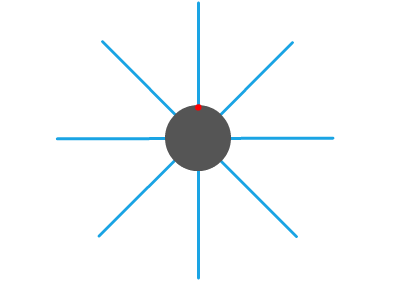
\includegraphics[width=\textwidth]{misc/sensors_wall.png}
\label{fig:sensors_wall}
\caption{A single robot seen from above. The lines emanating from the body represents the reach of the distance sensors.} 
\end{figure}

The robots also have a sensor that can sense if they are directly on top of an energy point. 
The sensory input the agents get are fed into the neural network that controls the actuators of the robots. 
There are four actuators: The two wheels, the "mouth" that absorbs food and the output that creates energy points. 
Each robot is controlled by an artificial neural network that has 13 inputs that will be connected to the robot's sensors. 

\subsection{Sensors and actuators}

The robot has 12 sensors that all provide numeric input to the control mechanism. 
The function of the each sensor is given below:

\begin{itemize}
\item{1-8: Distance sensors}
\item{9: Direction to nearest energy point}
\item{10: Distance to nearest energy point}
\item{11: Energy level}
\item{12: Dependent on scenario}
\end{itemize}

The robot has three actuators, two wheels used for locomotion and an output for the energy points.


 
\section{Artificial Neural Networks}


ANNs are computational entities that are inspired by how the brain does computation. 
In the brain, a network of neurons acquire knowledge through the body's receptors and maps the perceptions it receives to a given action. 
Learning is achieved by strengthening the inter neuron connections, known as synaptic weights. \cite{haykin_neural_1994} 

One of the key reasons using a neural network is beneficial in this problem is that one of the great advantages of neural networks is that contextual information is taken into consideration. 
All the neurons in the network are affected by what is happening on a global level and therefore a given response may be elicited according to context.
In this case, the choice of relinquishing energy should be affected by whether or not there are other robots nearby and perhaps also how closely they are related.

Artificial neurons have a series of inputs that are altered according to the weight of the input. This weight is analogous to the strength of the synaptic connection.
There is also often an extra input that is constant and is known as a bias-weight. The summation of this is fed to an activation function that determines the output of the neuron. The output of one neuron can be fed as part of the input to another neuron and this is how the network is built. A neuron can also use its own output as an input, effectively giving the neuron memory. 

The ANN that the robots are controlled by is a multi-layer perceptron with three hidden neurons and three output neurons.
The output neurons control each of the wheels and has a binary output that decides if energy should be dropped or not. 

\begin{figure}
\centering
\def\svgwidth{\columnwidth}
\input{defaultNetwork.pdf_tex}
\label{fig:nn_default}
\caption{ANN used by the baseline and kin selection}
\end{figure}

Figure ~\ref{fig:nn_default} shows the schematic drawing of the artificial neuron used by the robots in the baseline and the kin selection scenario. 
The unused sensor input is set to be 0 at all times. 


\begin{figure}
\centering
\def\svgwidth{\columnwidth}
\input{neuralNetwork.pdf_tex}
\label{fig:nn_seeking}
\caption{ANN used by the kin seeking/recognizing population}
\end{figure}

	

%\begin{figure}
%\centering
%\def\svgwidth{\columnwidth}
%\input{kinRecognitionNetwork.pdf_tex}
%\label{fig:nn_recognition}
%\caption{ANN used by the kin recognizing population}
%\end{figure}


The ANN for the kin recognition and kin seeking scenarios are show in figure ~\ref{fig:nn_recognition} and ~\ref{fig:nn_seeking} respectively. 

\section{The Evolutionary algorithm - mEDEA}

The evolutionary algorithm to be used needed to be both robust to change and have a fitness function that rewards survival and spreading of genes. 
The reason for this is that the algorithm should be designed to reward selfish individuals on the individual level so that the altruistic behaviour arises as an evolutionary 
response that increases inclusive fitness. 
For this reason the mEDEA-algorithm was chosen.
The mEDEA algorithm is presented in pseudo code in figure ~\ref{alg:medea}
\begin{algorithm}[H]
\caption{The \textsc{mEDEA} algorithm}
{
\begin{algorithmic}[1]
 \STATE $genome$.\textcolor{red}{randomInitialize()}
 \WHILE{forever}
   \IF { $genome$.notEmpty() }
     \STATE agent.load($genome$)
   \ENDIF
   \FOR { $iteration$ = 0 to \textcolor{blue}{$lifetime$} }
     \IF { $genome$.notEmpty() }
       \STATE agent.move()
       \STATE \textcolor{blue}{broadcast}($genome$)
     \ENDIF
   \ENDFOR
   \STATE $genome$.empty()
   \IF { \textit{genomeList}.size $>$ 0 }
     \STATE $genome$ = \textcolor{red}{applyVariation}(\textcolor{red}{$select_{random}$}(\textit{genomeList}))
     \ENDIF
     \STATE \textit{genomeList}.empty()
 \ENDWHILE
 \end{algorithmic}
}
\label{alg:medea}
 \end{algorithm}

In the mEDEA algorithm each agent has a list of genomes. 
Every time an agent encounters another agent they add that agent's genome to their list of genomes and when an agent is reactivated it chooses a genome from it's list of genomes that will serve as the basis for the new genome of the agent. 
The genomes are mutated as in regular evolutionary algorithms and the selection scheme can also vary. 
The fact that survival and dissemination of genes is an implicit demand of the mEDEA algorithm makes it a great fit for the experiment. 
The mEDEA-algorithm has an implicit fitness function. 
The better the individuals are at spreading their genes, the greater are their chances to pass on their genes. 
This closely mimics the way evolution works in real life.  
Having an implicit fitness function that partially rewards for the trait we are after is having traits appear by design rather than by necessity. 
An agent is deactivated when it runs out of energy and reactivated when another agent passes nearby.


\begin{figure}[H]
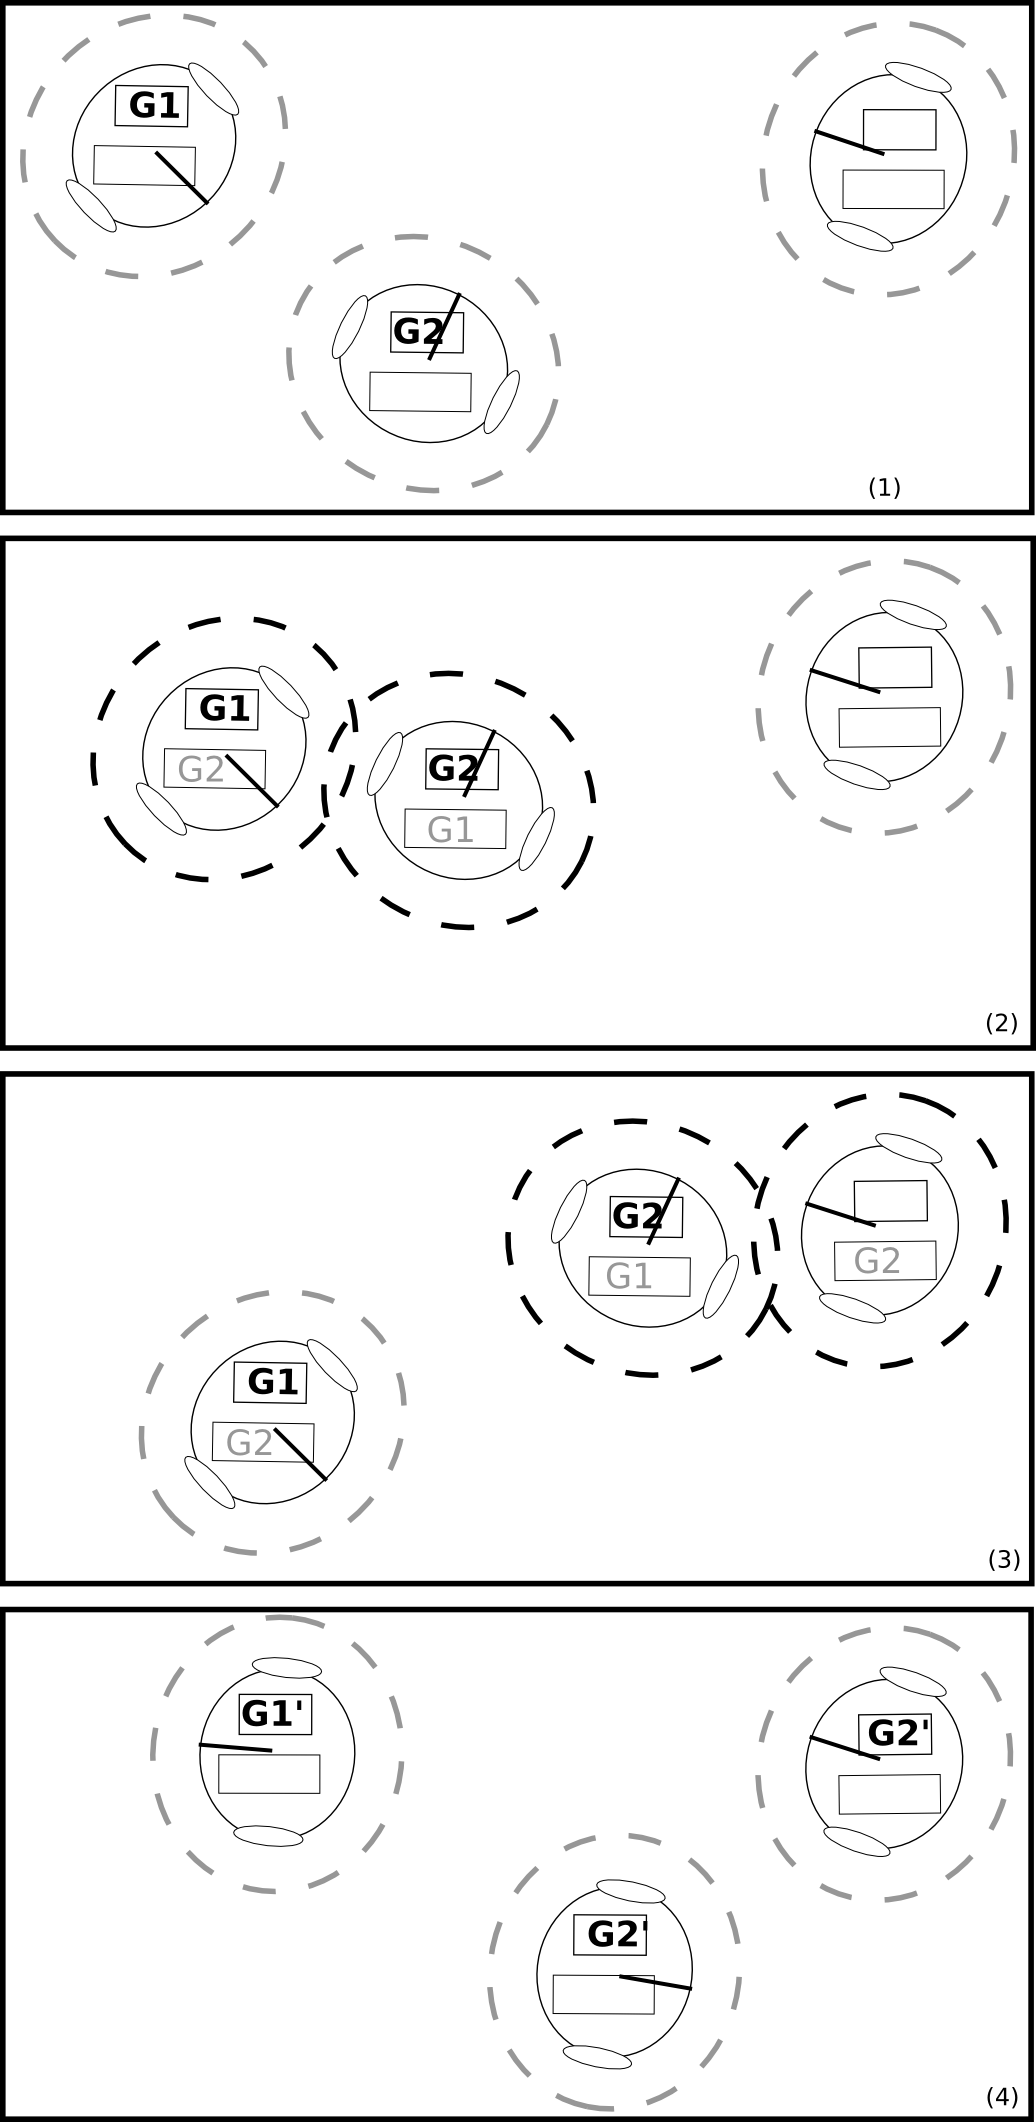
\includegraphics[height= \textheight]{misc/medea.png}
\caption{Sequence showing how genomes are exchanged in the mEDEA-algorithm}
\label{fig:medea}
\end{figure}

\section{Donating Energy}
The agents each have an output neuron that outputs a floating point value. If the value is above a predetermined threshold the agent creates an energy point in the environment that 
it cannot utilize for itself. The energy points that are created are never replenished unlike the energy points that are intrinsic to the environment. The amount of energy donated is set to be a predetermined number. This was chosen to simplify the experiments, but ideally the amount of energy donated should be determined by the output value of the neuron.

Using a predetermined value relieves the model of biological accuracy, but it allows for greater control and understanding of the parameters 
that are needed for the wanted behaviour to occur, which is the object of the experiment. Early initial tests showed that linking the amount of energy donated in each time step unsurprisingly 
led to the first generation of agents committing mass suicide in the first few time steps since the output value from the beginning is random. It is a reasonable to assume that the insects or
animals the robots model already have evolved an inclination towards not dropping food and that this should only happen when a certain sensory input is provided.   

\subsection{The environment}
The environment the robots inhabit is a large two dimensional square with a few obstacles scattered around. 
Very little exists in the environment and the robots roam around freely.
A screen shot of the environment can be seen in figure % ~\ref{fig:initialPeriod} 

  
\begin{figure}[H]
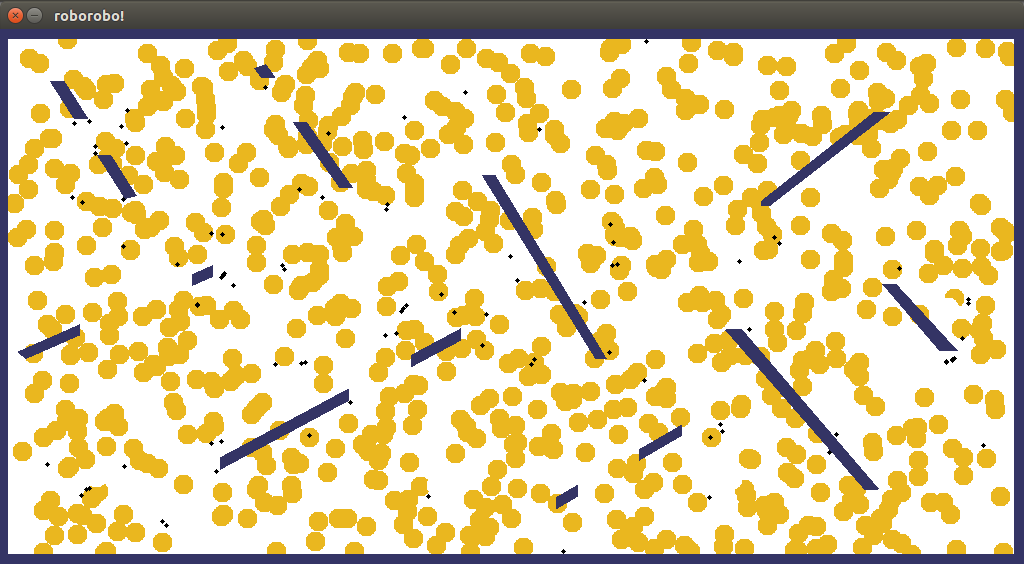
\includegraphics[width=\textwidth]{misc/initialPeriod.png}
\label{fig:initialPeriod}
\caption{Screen shot of the robots in the initial period. The colored dots are the the energy points created by the environment, the black dots are robots and the lines are walls}
\end{figure}

\section{Important parameters for the initial period }

The complete properties file for the experiment can be found in the appendices. 

The robots start out with a total of 100 units of energy and a generation lasts 400 iterations.
1 unit of energy is spent per iteration which gives the genome 1/4 of generation to prove itself.


\begin{table}[H]
\begin{center}
\begin{tabular}{|l|c|}\hline
Energy expenditure    &  1 \\\hline\hline
Initial energy 		& 100 \\\hline\hline
Iterations/generation & 400 \\\hline\hline
Energy points & 100 \\\hline\hline
Energy point value & 50 \\\hline\hline
Revival energy & 400 \\\hline\hline
\end{tabular}
\end{center}
\label{table:parameteres}
\caption{Important parameters for the first experiment}
\end{table}
  
\section{Important parameters for the final period}


The threshold that the output of the donation neuron needs to exceed for a donation to occur is set to 0.5.
Since the initial output value of this neuron is not a factor in the initial evolution of the agents it is to be expected that half of the agents will become donors immediately and the other half won't 
Introducing the trait in this way is artificial but it if the trait has a negative enough impact on the fitness of the individuals the trait will soon disappear. 
The energy expenditure in the altruism part of the experiment is set to 0.005 per iteration. 
The initial energy of the robot is set four times higher than in the initial period so that there will be enough time for the altruistic agents to meet other agents and propagate their genes as the initial tests showed that the altruistic agents would often give away so much energy in the beginning causing them to die out before being able to spread their altruistic genes.
This also caused the entire population to go extinct shortly after.
In this second period the robots spend 0.005 per iteration which makes the total expenditure of energy per generation 20 units for each agent. This means that they can survive for 200 generations without needing food provided they don't donate energy. 
This value is set low to ensure that the agents survive long enough that evolution can occur. 

For the first experiment the number value of each energy point to be generated by each agent was set to be 50. 
This means that the agents can run out of energy if they create more than 16 energy points in the first generation.
This number was chosen to be low enough that not all agents that are inclined to donate energy will die, but 
high enough so that the energy point provides useful sustenance for other agents. 

The experiment is run for 400 generations to see what happens when the robots are close to running out of energy altogether, but the main period of interest is before this when the agents need to distribute the energy they have among them in order to ensure that all the active agents survive as long as possible.


\begin{table}[htdp]
\begin{center}
\begin{tabular}{|l|c|}\hline
Donation Threshold    &  0.5  \\\hline\hline
Energy Point value    &  50  \\\hline\hline
Energy expenditure    &  0.005 \\\hline\hline
Initial energy 		& 400 \\\hline\hline
Iterations/generation & 400 \\\hline\hline
\end{tabular}
\end{center}
\label{table:parameteres2}
\caption{Important parameters for the final period}
\end{table}
\section{Experimental setup}

All the experiments were run on an Intel Centrino 2 clocked at 2.26 MHz. For each setting, each experiment was run 100 times and the results computed as an average over those runs. 
On average, a single complete run of one experiment with both the initial period and the final period took approximately 30-35 minutes. 
To implement the experimental environment described an existing system that fulfilled many of the requirements was modified.
The system that was used was Roborobo which is a 2D robot simulator based on the epuck/kephra model written mainly by Nicolas Bredeche with assitance from Jean-Marc Montanier and Leo Cazenille. Roborobo is written in C++ and is described in detail in \cite{roborobo}
This system was chosen because it was available in open source and because it provided a lot of the functionality that was needed for the experiment:

\begin{itemize}
  \item Ready made environment for simulating small robots
  \item	Integrated code for neural networks
  \item Built-in evolutionary algorithm functionality  \ldots
\end{itemize}

The graphs were created using the Java library JFreeChart available at \url{http://www.jfree.org/jfreechart/}


\chapter{Results}
\label{cha:results}

In this chapter the results from the experiments are presented. 
First the results of the baseline is presented to show the behaviour that is expected when no kin-recognition is present in the system
The results from the three experiments are presented in turn and the same graphs are shown for all the experiments.

\begin{itemize}
\item The amount of agents over time
\item The amount of agent generated points created and consumed
\item The amount of energy available in agents and points
\end{itemize}

For all graphs the standard deviation is shown as a shaded area beneath the plot.

\section{Baseline}

%figure baseline agents.

\begin{sidewaysfigure}
	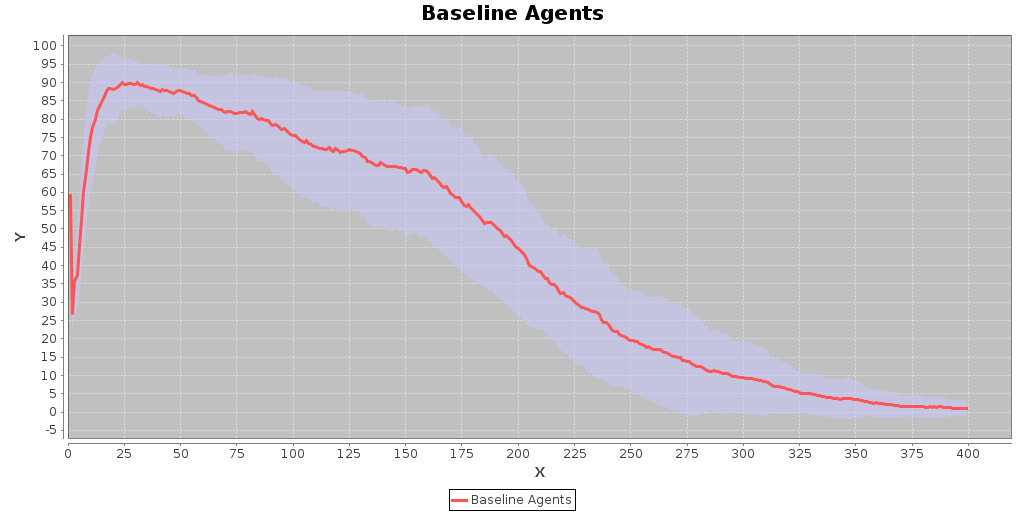
\includegraphics[width=\textwidth]{expr2/baseline_agents.png}
    \caption{Graph showing the number of active robots in each generation for the baseline}
    \label{fig:agents_baseline}
\end{sidewaysfigure}

\begin{sidewaysfigure}
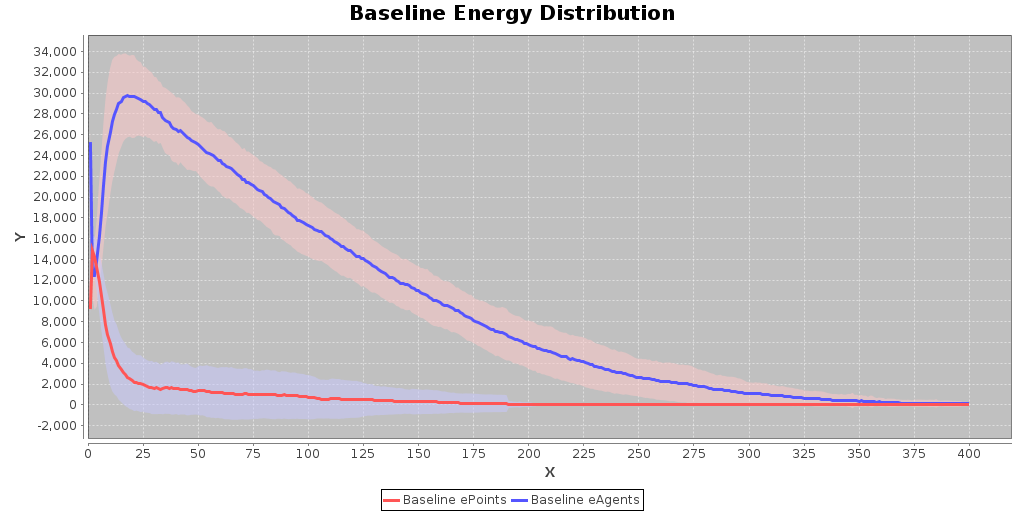
\includegraphics[width=\textwidth]{expr2/baseline_distribution.png}
    \caption{Graph showing the amount of energy in the system and the amount of energy in the robots for the baseline}
\label{fig:distribution_baseline}
\end{sidewaysfigure}

\begin{sidewaysfigure}
	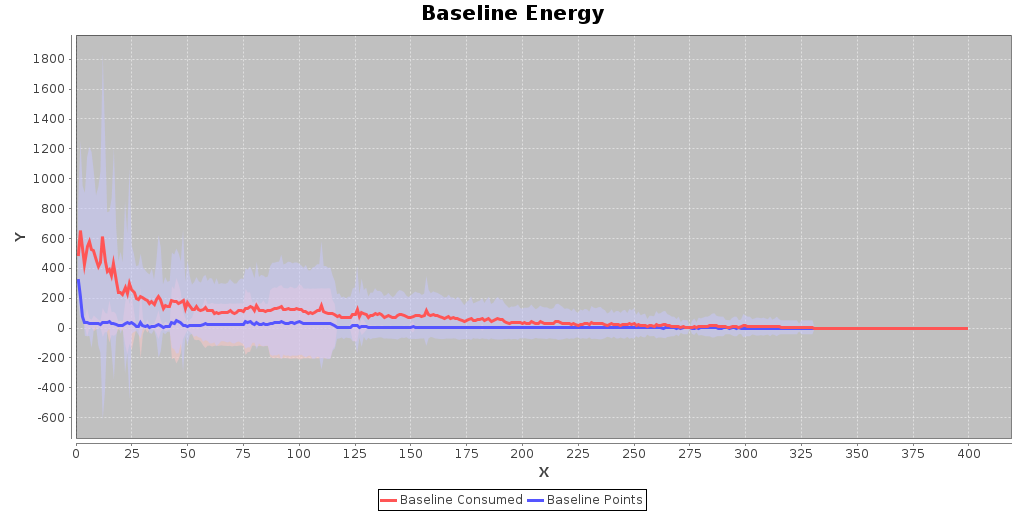
\includegraphics[width=\textwidth]{expr2/baseline_energy.png}
    \caption{Graph showing the number of points created and consumed each generation for the baseline}
    \label{fig:points_baseline}
\end{sidewaysfigure}



Figure ~\ref{fig:agents_baseline} shows the graph displaying the number of active robots in the environment at the end of each generation.
The number of robots first drops dramatically as there is an extreme amount of self sacrifice in the begin when the donations happen at random.
The number of robots quickly rises again as the remaining active robots who are not giving away energy consume the energy that has been dropped.
The robots then gradually become inactive as the robots with the least amount of energy expend all their energy while there is less and less energy 
available in the environment as shown in figure ~\ref{fig:distribution_baseline} which shows the sum total of energy in the robots and the sum total of energy in energy points in the environment over time.
Figure ~\ref{fig:points_baseline} shows the number of points created and consumed. It is clear that after the initial period there is very little energy being brought into the environment as very few new energy points are created. 



\section{Kin recognition}
\label{sec:recog}

\begin{sidewaysfigure}
	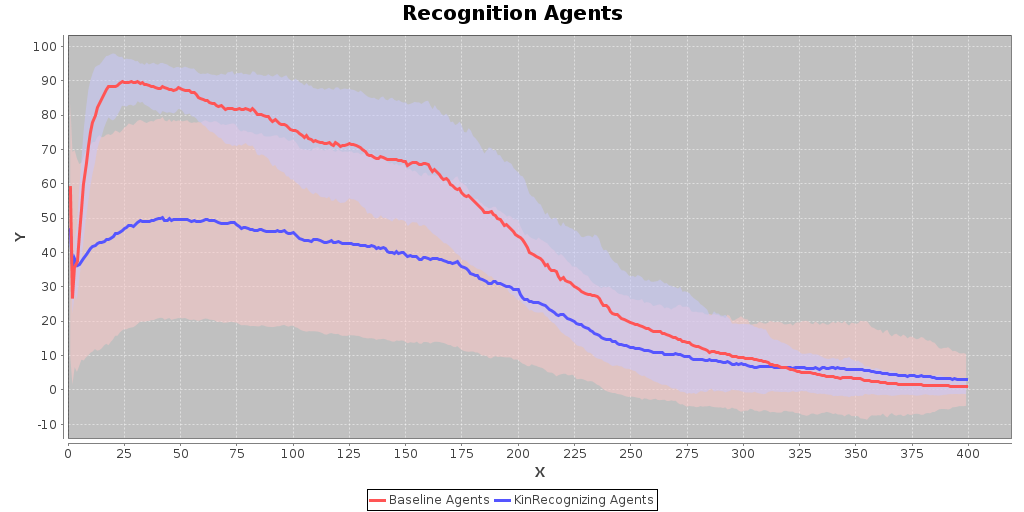
\includegraphics[width=\textwidth]{expr2/recognition_agents.png}
    \caption{Graph showing the number of active robots in each generation for the kin recognition scenario}
    \label{fig:agents_recognition}
\end{sidewaysfigure}

\begin{sidewaysfigure}
	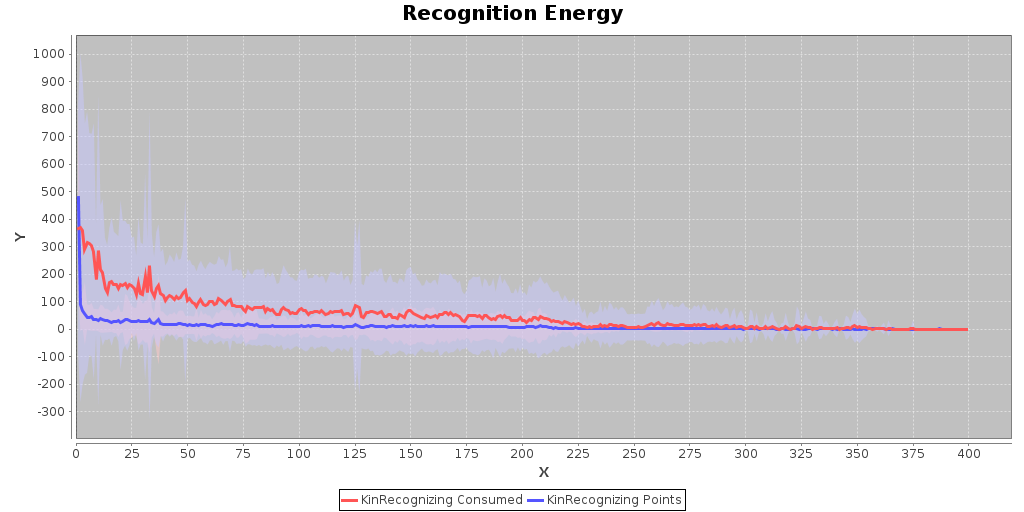
\includegraphics[width=\textwidth]{expr2/recognition_energy.png}
    \caption{Graph showing the number of points created and consumed each generation for the kin recognition scenario}
    \label{fig:points_recognition}
\end{sidewaysfigure}

\begin{sidewaysfigure}
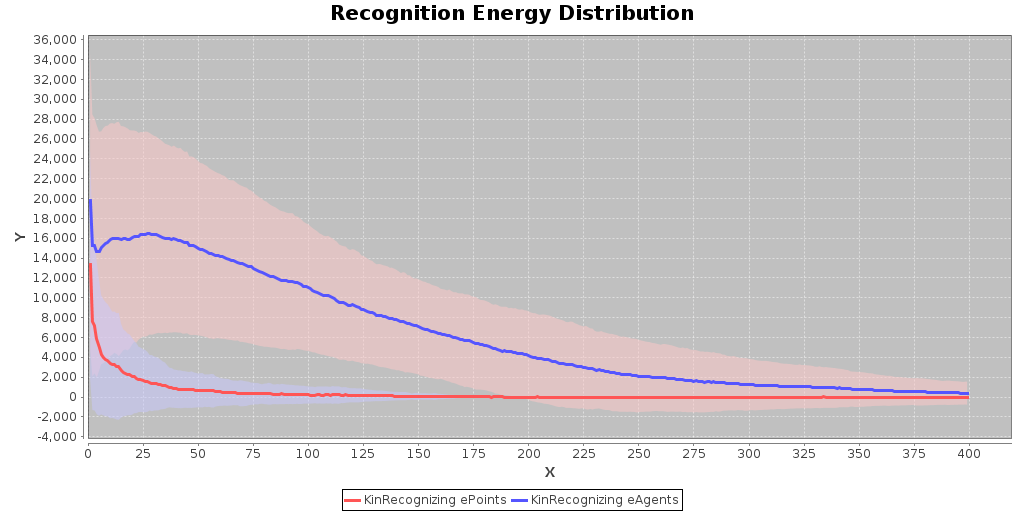
\includegraphics[width=\textwidth]{expr2/recognition_distribution.png}
    \caption{Graph showing the amount of energy in the system and the amount of energy in the robots for the kin recognition scenario}
\label{fig:distribution_recognition}
\end{sidewaysfigure}

Figure ~\ref{fig:agents_recognition} shows the graph with the number of active robots in the kin recognition scenario superimposed on the graph with the number of active robots in the baseline from ~\ref{fig:agents_baseline} for reference. 
The drop in number of robots is less dramatic than in the baseline, but in return the rise in number active agents in the subsequent period is substantially less. 
The cause of this is unknown, an hypothesis could be that the kin seeking population is more homogeneous than the baseline. 
This could lead to less of an impact on the population because the surviving robots have a similar genetic make-up as the ones that die, so more robots keep on creating energy points after the initial period. 
The graph in figure ~\ref{fig:points_recognition} supports this by showing that roughly 50 \% more points are created in the first 25 generations which is the time it takes the baseline to reach its maximum population. 
There were however no measurements of the homogeneity of the populations at the start of the second period made that can be used to support this.
The graph in figure ~\ref{fig:distribution_recognition} shows that for a large section of the duration of the experiment the amount of energy in the system is constant although points are being consumed. 

\section{Kin seeking}

Kin seeking writeup
\begin{sidewaysfigure}
	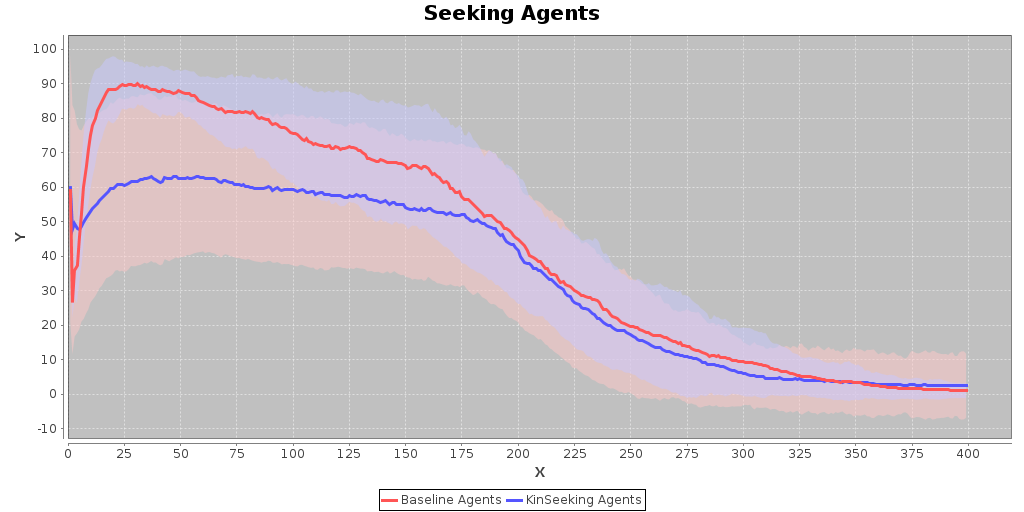
\includegraphics[width=\textwidth]{expr2/seeking_agents.png}
    \caption{Graph showing the number of active robots in each generation for the kin seeking scenario}
    \label{fig:agents_seeking}
\end{sidewaysfigure}

\begin{sidewaysfigure}
	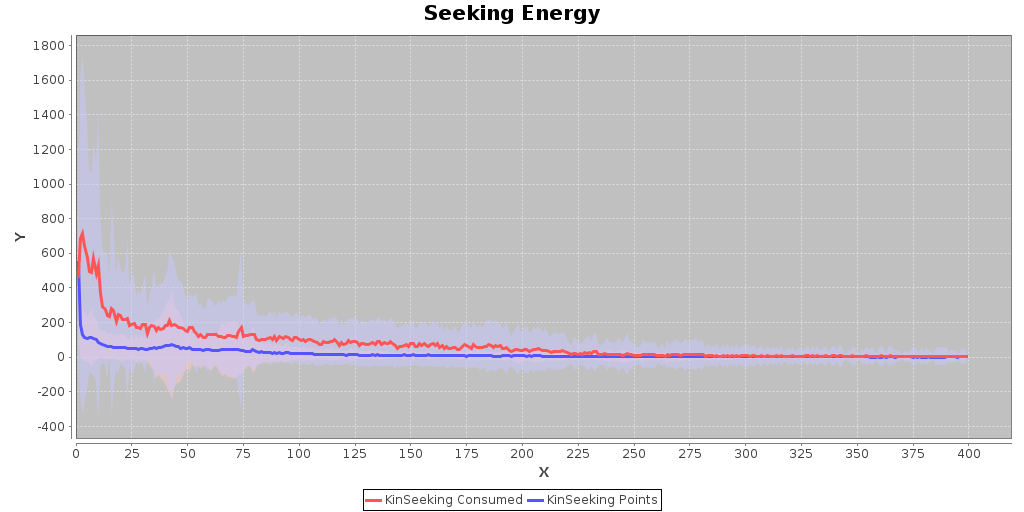
\includegraphics[width=\textwidth]{expr2/seeking_energy.png}
    \caption{Graph showing the number of points created and consumed each generation for the kin seeking scenario}
    \label{fig:points_seeking}
\end{sidewaysfigure}

\begin{sidewaysfigure}
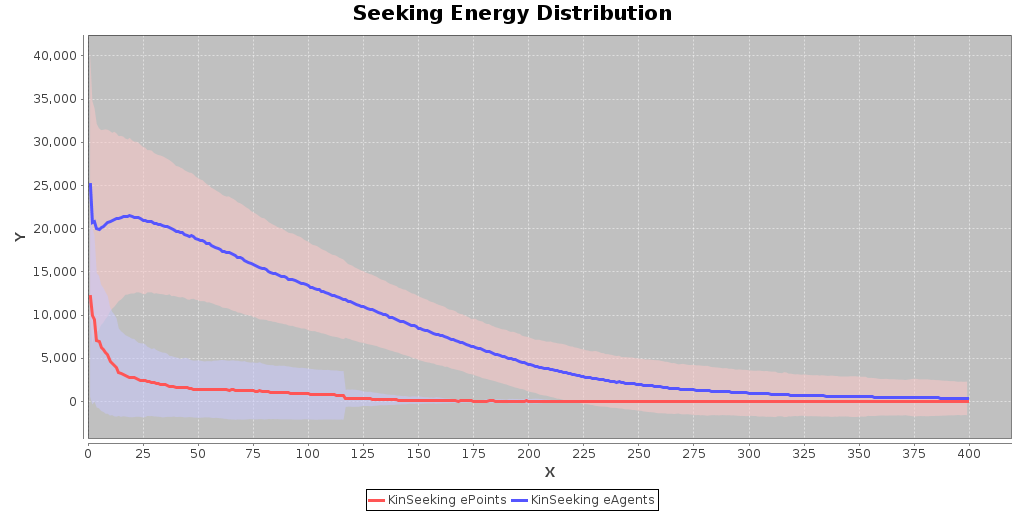
\includegraphics[width=\textwidth]{expr2/seeking_distribution.png}
    \caption{Graph showing the amount of energy in the system and the amount of energy in the robots for the kin seeking scenario}
\label{fig:distribution_seeking}
\end{sidewaysfigure}

Figure ~\ref{agents_seeking} shows the same graph as in figure ~\ref{agents_recognition} for the kin seeking scenario.
The shape of the graph is very similar to that of the kin recognition scenario shown in ~\ref{sec:recog} only shifted upwards on the y-axis, having approximately 10 more active roots on average. The mechanisms behind the shape itself is thought to be similar to that of the kin recognition graph and the cause of the shift is simple. The graph in ~\ref{seeking_energy} reveals that more energy points are created in the kin seeking scenario. The reason for this is unclear, but the hypothesis is that there is an even more homogeneous population evolved in the initial period in the kin seeking scenario.   

\section{Kin selection}

kin selection writeup

\begin{sidewaysfigure}
	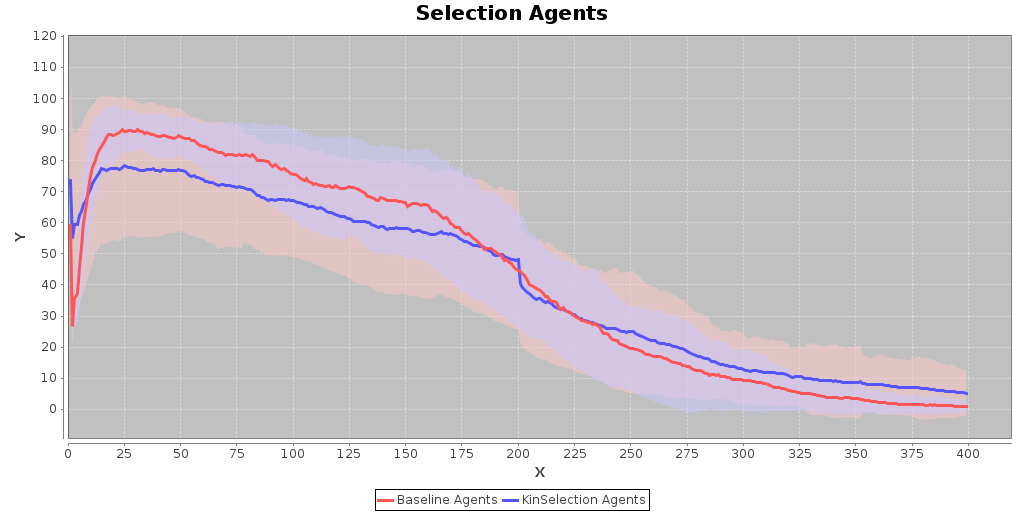
\includegraphics[width=\textwidth]{expr2/selection_agents.png}
    \caption{Graph showing the number of active robots in each generation for the kin selection}
    \label{fig:agents_selection}
\end{sidewaysfigure}

\begin{sidewaysfigure}
	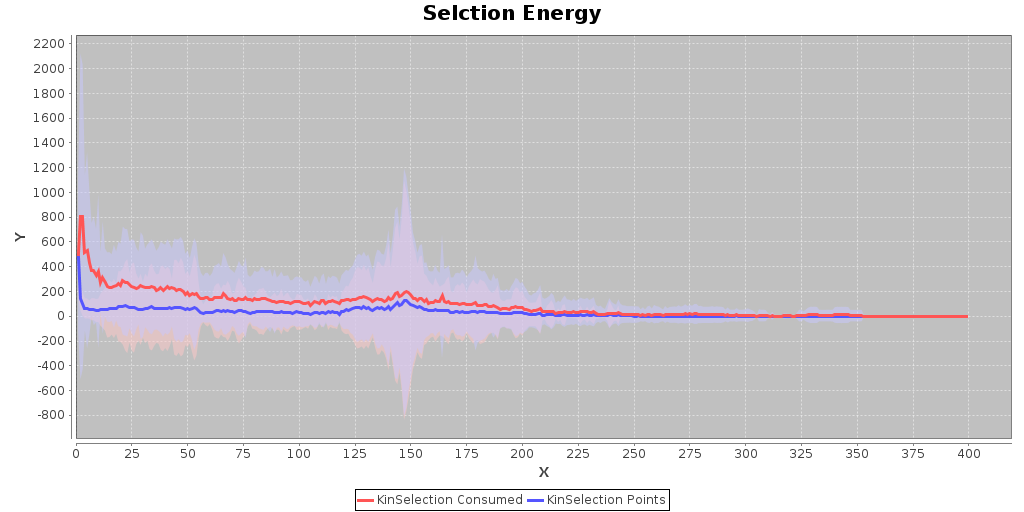
\includegraphics[width=\textwidth]{expr2/selection_energy.png}
    \caption{Graph showing the number of points created and consumed each generation for the kin selection}
    \label{fig:points_selection}
\end{sidewaysfigure}

\begin{sidewaysfigure}
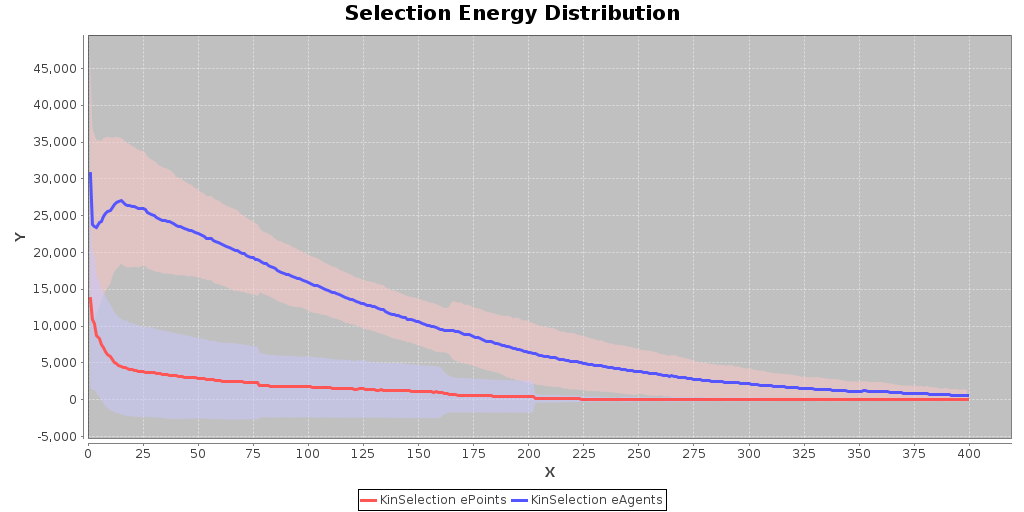
\includegraphics[width=\textwidth]{expr2/selection_distribution.png}
    \caption{Graph showing the amount of energy in the system and the amount of energy in the robots for the kin selection}
\label{fig:distribution_selection}
\end{sidewaysfigure}

\section{Graph overlay}

When putting all the graphs on top of each other as can be seen in figure ~\ref{fig:agents_overlay} the effect of the kin oriented algorithms become visible. 
The number of active agents never rise to the same level as in the baseline with the maximum number among the kin oriented algorithms at 45 active robots opposed to nearly 70.
However, the amount of agents drops a lot more rapidly in the non-kin oriented algorithms and soon after a 100 generations all the kin oriented populations are more successful. 


\begin{sidewaysfigure}
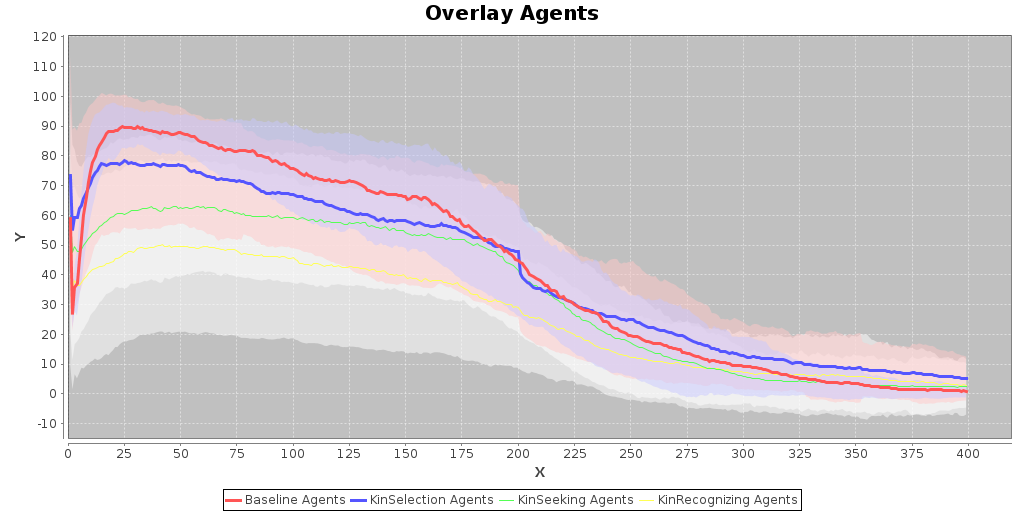
\includegraphics[width=\textwidth]{expr2/overlay_agents.png}
    \caption{Graph showing the number of agents in all the runs}
\label{fig:agents_overlay}
\end{sidewaysfigure}


\begin{sidewaysfigure}
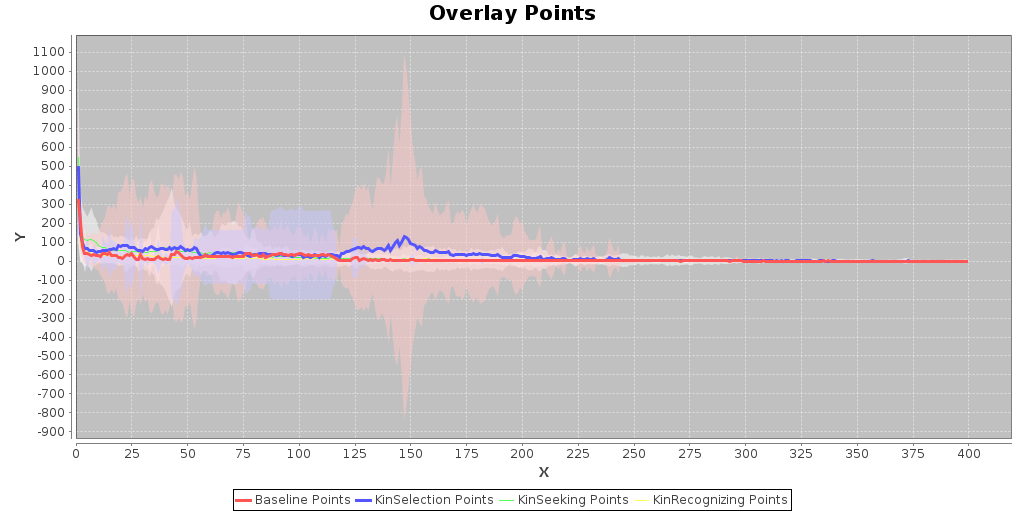
\includegraphics[width=\textwidth]{expr2/overlay_points.png}
    \caption{Graph showing the number of agents in all the runs}
\label{fig:points_overlay}
\end{sidewaysfigure}

Figure ~\ref{fig:points_overlay} shows the overlay of the number of points created. 
The kin seeking population creates slightly more energy points than the others explaining why they remain the most successful population for a large portion of the experiment.
In the period from 120 to 170 the kin selection population creates more points than the others which explains why it ends up as the most successful population towards the end of the simulation. A detail of this is shown in figure ~\ref{fig:detail_points_overlay}

\begin{figure}
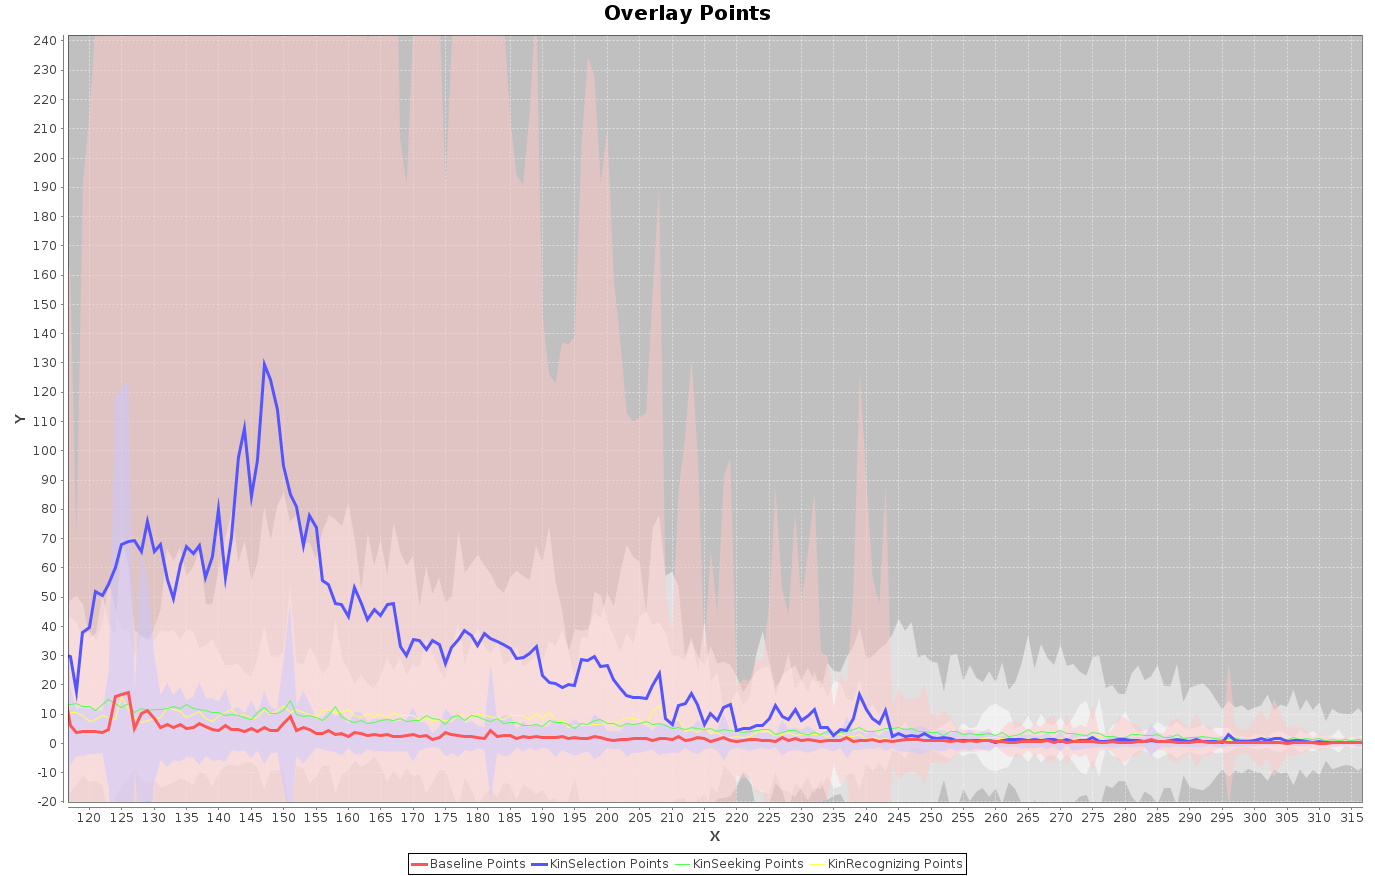
\includegraphics[width=\textwidth]{expr2/overlay_points_detail}
\caption{Overlay graph of the number of points created for each scenario}
\label{fig:detail_points_overlay}
\end{figure}
\chapter{Discussion}

This chapter contains of the results presented in the previous chapter and addresses the implications they have regarding the research question.

\section{How successful were the kin oriented mechanisms?}

All the kin mechanisms have more robots alive than the baseline after the initial period of 100 generations and all the kin mechanisms have on average more robots alive at the end of the 400th generation. A contributing factor to this could simply be that the baseline has a much larger population during the first 100 generations and this more energy is spent and less energy is available to the remaining generations. It's difficult to say why the baseline donates much more energy than the other populations in the beginning and it could be due to an error in the model although no error has been found. 

\section{Similarities of kin seeking and recognition}
The graphs displaying the number of active agents reveals that the shape of the curves for kin seeking and kin recognition look remarkably similar. 
The detail of the graph shown in figure ~\ref{fig:recogdetail} shows that they display the same pattern of falling before rising slightly and then falling again before they ascend to the highest point. This could be an indication that the populations evolved by the kin seeking population and the kin recognizing population may have a similar constitution.

\begin{figure}[H]
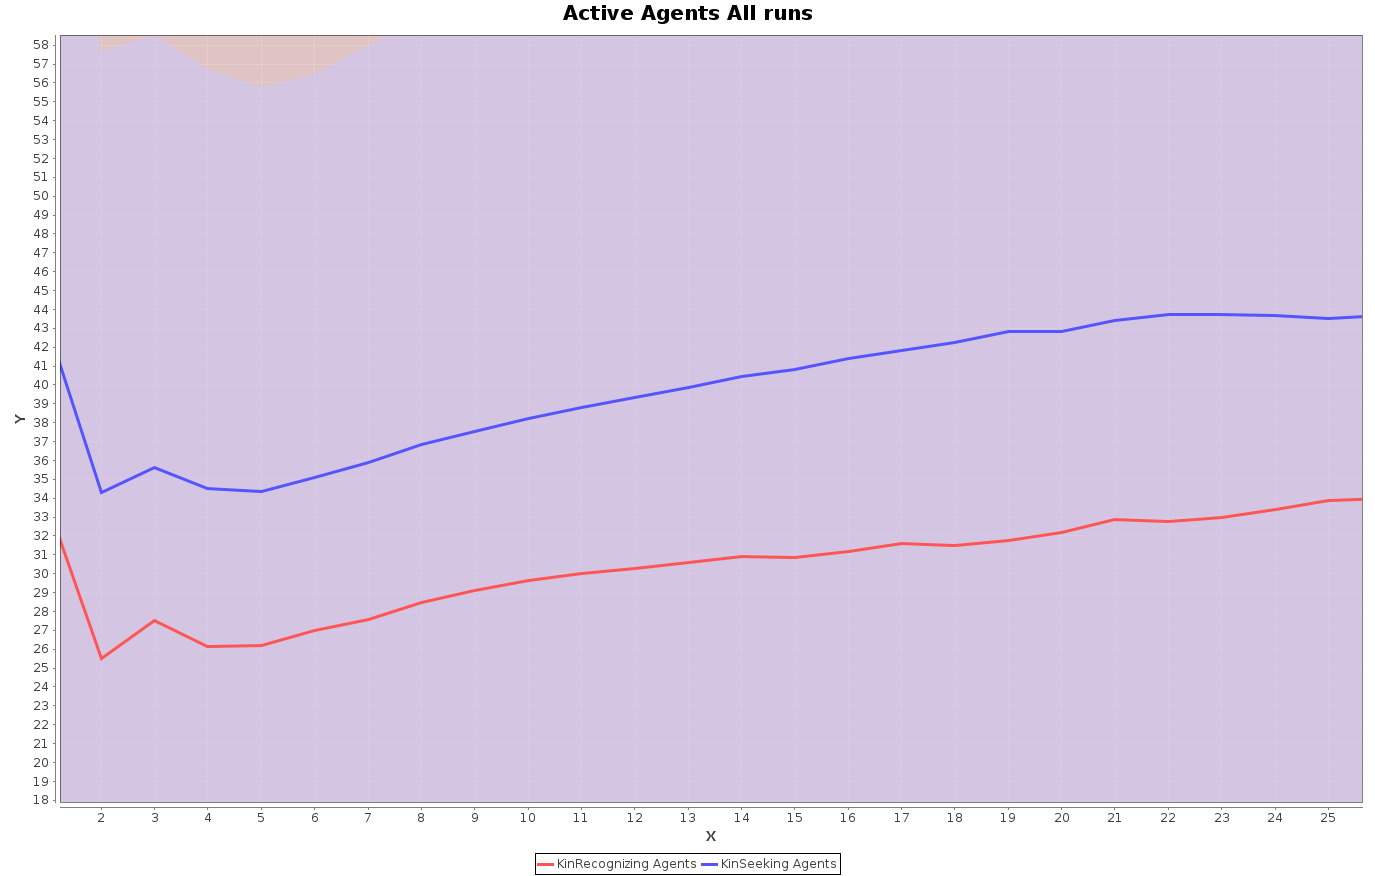
\includegraphics[width=\textwidth]{expr1/recogVSseekingDetail.png}
\label{fig:recogdetail} 
\end{figure}

\section{Future work}

The results from the experiments leave room for much to be explored. 
This section gives a few suggestions on what should be pursued further.

\subsection{More advanced version of kin seeking algorithm}
The kin seeking algorithm seems promising and it would be interesting to run an experiment where the robots are given the direction of the largest concentration of related individuals.
In this scenario the robot may seek out a group of robots that has a similar genotype. 
The hypothesis is that this would lead to more robots with altruistic inclinations profiting from the altruism when altruistic individuals group together. 
The challenge would be to find a purposeful way of grouping the robots together when assessing which area has the largest concentration of related individuals. 
One way of doing this could be to partition the environment into sections where the average degree of relatedness is calculated for each agent for each section. 
However, this method makes it more challenging to transfer the method to situated agents as it requires each of the robots to have a mapping function. 
Assuming the robots broadcast their whereabouts this could be solved by sectioning a circle surrounding the agents.

\subsection{More advanced version of the kin recognizing algorithm}
The kin recognizing algorithm could be expanded upon by having the agents take into account how related the are to all agents that are within close enough distance to transfer their own genome. 
This could provide a higher chance that the robots would give away energy when related agents are close enough that they may benefit from the donation.
Another benefit of this method is that it makes use of the already necessary functionality in the robots to broadcast their genome to all agents who are close enough.
This makes it a more practical method than the kin seeking method as less elaborate methods of 

\subsection{Tracking of population composition}
A likely hypothesis is that the difference in the amount of energy donated to the environment is connected to how homogeneous the population is.
Future work could involve tracking the homogeneity of the population as a whole to see how it coincides with the donation of energy, if there is any correlation at all.
This tracking could involve tracking the homogeneity of local groups in the population where the energy points are being created to see if there is a difference in the sub groups in the environment.
If it can be shown that some local groups produce altruists a challenge would be to device a mechanism for spreading these genes since high viscosity contributes to the development of altruism.



\section{Energy transferring}
In the experimental set up used the robots donate energy to the environment without any assurance that the energy is consumed by the intended beneficiary.
This increases the chance that related individuals will be deprived of the energy and in as a consequence giving away energy is less likely to increase the inclusive fitness.
In future experiments the way of donating energy could be changed to a direct transfer of energy between the robots. T
his would eliminate the problem and also provide a higher degree of realism since creating a way to exchange energy between actual robots would be best devised with a form of aggregation or through wireless energy transmission. In both cases, proximity is a factor that must be taken into account. 

\begin{appendices}

\chapter{Systematic Literature Review Protocol}\label{T-B}
\label{cha:STL}
%\chapter{Evolving Self-Sacrifice: A Systematic Literature Review}\label{T-B}
%\label{cha:STL}

%\section{Introduction}
%\label{sec:STLintro}


The systematic literature review was performed using the guidelines for systematic 
literature review in software engineering presented in \cite{keele_guidelines_2007}.
The review protocol is presented along with the documentation of each step.
The literature review process is divided into 8 steps: %Check Kitchenham 2007

\begin{description}
\item[Step 1] {\it Defining review questions}

\item[Step 2] {\it Defining the systematic literature review protocol}

\item[Step 3] {\it Search for relevant studies}

\item[Step 4] {\it Selection of studies}

\item[Step 5] {\it Quality assessment}

\item[Step 6] {\it Data Collection}

\item[Step 7] {\it Data synthesis and analysis}

\item[Step8] {\it Dissemination}

\end{description}

\clearpage 

\section{Defining the Review Questions}
The first step in the systematic review process was to formalize the the goal of the review into review questions that the review is meant to answer. The goal of the review was to answer the following questions:

\begin{description}
\item[RQ1] {\it What are the mechanisms that allow altruistic behavior to evolve?} 
\item[RQ2] {\it What are the most important factors in determining the degree of altruism displayed?}
\item[RQ3] {\it Which methods show the most promise in achieving self sacrificial behaviour in artificial evolution?}

\end{description}

%\subsection{Defining the Systematic review Protocol}

%I'm not sure what to write here as I'm detailing the protocol as I go along.

\section{Search for Relevant Studies}

To perform the search in a systematic way I compiled a list of of relevant sources which would be the subject to systematic query. I decided to use the list compiled in \cite{Lillegraven_design_2010} as a starting point as it presented a list of relevant sources both for research on computer science in general and had already been used to find sources in Artificial Intelligence. 
%In Addition to the sources identified there I also added Google Scholar and Science Direct as suggested by 
%\cite{Brereton_lessons_2007}. Google Scholar would be my primary source in identifying relevant papers The list of sources is shown in table \ref{table:sources}


\begin{table}[htdp]
\begin{center}
\begin{tabular}{|l|c|r|}\hline
Source                  &   Type                        & URL \\ \hline \hline
ACM Digital Library     &   Digital Library             & \url{http://portal.acm.org/dl.cfm} \\  \hline %Subscription
IEEE Xplore             &   Digital Library             & \url{http://ieeexplore.ieee.org/} \\ \hline   %Subscription
CiteSeerX               &   Digital Library             & \url{citeseerx.ist.psu.edu} \\ \hline         %Free
Web of Knowledge        &   Digital Library             & \url{http://wokinfo.com/} \\ \hline           %Free
%    Google Scholar          &   Bibliographic Database      & \url{http://scholar.google.com} \\ \hline     %Free
Journal of AI Research   &   Journal                     & \url{http://jair.org/} \\  \hline      %Free
References in papers    &   N/A                         & N/A \\\hline\hline
\end{tabular}
\end{center}
\label{table:sources}
\caption{Sources considered in the online search}
\end{table}
\subsection{Searching the online resources }
Following the methodology in \cite{oates_researching_2005} I created groups of search terms that were synonyms or similar in meaning. The purpose of this was to exploit the possibility of using boolean search strings in modern digital libraries. 
The search for relevant literature is a continuous process and I went through a number of different tables of search terms. 
The table of search terms presented in table \ref{table:terms2} is the one I ended up using. The sparsity of the table is a conscious choice as having a general search query and then narrow the results down based on research subject proved a more effective method for finding relevant literature.
The search terms were combined in the boolean search string in equation \ref{eq:search2}
%\begin{center}
%   \begin{tabular}{| l | c | c | r |}
%     \hline
%      & Group 1 & Group 2 & Group 3 \\ \hline
%      Term 1 & Altruism & Evolution & Swarm Robots \\ \hline
%      Term 2 & Tragedy of Commons & Natural Selection & Swarm Intelligence \\ \hline
%      Term 3 & Collaboration & Evolving & Swarm Behavior \\ \hline
%      Term 4 & & Evolutionary & \\ \hline
%      Term 5 & & Genetic & \\
		%      \hline
		%       \label{table:terms1}
		%       \end{tabular}
		%end{center}
		%     
		%his provided me with a set of 
		%
		%begin{equation}
		%label{eq:comb}
		%*5*3 = 60
		%end{equation}
		%
		%\noindent
		%combinations of search terms. Combining the different search terms created the search string in \ref{eq:search}
		%\noindent
		%begin{multline}
		%label{eq:search}
		%"Swarm Behavior" \lor "Swarm Robotics" \lor "Swarm Intelligence") \land \\
			%Evolutionary \lor Evolution \lor Evolving \lor Natural Selection \lor Genetic) \land \\
			%Altruism \lor Altruistic \lor Tragedy of Commons) \\
			%end{multline}
			%
			\begin{table}[htdp]
			\begin{center}
			\begin{tabular}{| l | c | r |}
			\hline
			& Group 1 & Group 2 \\ \hline
			Term 1 & Altruism 	& Evolution  \\ \hline
			Term 2 & Self-Sacrifice	& Natural Selection \\ \hline
			Term 3 & 		& Evolving   \\ \hline
			Term 4 & 		& Evolutionary  \\ \hline\hline
			\end{tabular}
			\end{center}
			\label{table:terms2}
			\caption{Search terms used}
			\end{table}
			%This provided me with a set of 
			%\begin{equation}
			%\label{eq:comb2}
			%2*4 = 8 
			%\end{equation}

			%\noindent
			%pairs of combinations of search terms that was combined as shown in \ref{eq:search2}


			%\begin{center}
			%    \begin{tabular}{| l | c | c | r |}
			%      \hline
			%       & Group 1 & Group 2 & Group 3 \\ \hline
			%       Term 1 & Altruism & Evolution & Kin-selection\\ \hline
			%       Term 2 & Altruistic & Natural Selection & Viscosity\\ \hline
			%       Term 3 & Self-sacrifice & Evolving &  \\ \hline
			%     Term 4 & & Evolutionary & \\ \hline
			%      \hline
			%	\label{table:terms1}
			%	\end{tabular}
			%\end{center}

			%This provided me with a set of 

			%\begin{equation}
			%\label{eq:comb2}

			%2*4*2 = 16 

			%\end{equation}

			%combinations of search terms combined in the boolean expression:

			\begin{center}
			\begin{multline}
			\label{eq:search2}
			(Altruism \lor Altruistic ) \land \\
				(Evolution \lor Natural Selection\ \lor Evolving \lor Evolutionary)
				\end{multline}
				\end{center}
				%\subsection{Searching offline}
				%To limit the number of results, the search was set to only return results published
				%in the last 5 years. The rationale was that this field of research is still in
				%its infancy and that the most relevant studies would be the most recent. This turned 
				%out to be a wrongful assumption, and later iterations did not limit the search
				%based on year of publication.

				\subsubsection{ACM Digital Library}
				For the ACM Digital Library, the number of results on the original search query
				was so large that it had to be further limited by only including entries from 
				relevant publications. Of the publications that returned matches for the query,
				these were included in the final search:

				\begin{itemize}

				%\item{Proceedings of the 13th annual conference companion on Genetic and evolutionary computation (255)}
				%\item{Proceedings of the 11th International Conference on Autonomous Agents and Multiagent Systems - Volume 3 (175) }
				%\item{The 10th International Conference on Autonomous Agents and Multiagent Systems - Volume 3 (171)}
				\item{Proceedings of the 9th annual conference on Genetic and evolutionary computation}
				\item{Proceedings of the fourteenth international conference on Genetic and evolutionary computation conference companion}
				\item{Proceeding of the fifteenth annual conference companion on Genetic and evolutionary computation conference companion}
				\item{Autonomous Agents and Multi-Agent Systems}
				\item{Evolutionary Computation}
				\item{Proceedings of the fourth international joint conference on Autonomous agents and multiagent systems}
				\item{Proceedings of The 8th International Conference on Autonomous Agents and Multiagent Systems - Volume 2 }
				\item{Artificial Life and Robotics}
				\item{Proceedings of the 2004 international conference on Multi-Agent and Multi-Agent-Based Simulation }
				\item{Proceedings of the Twenty-Second international joint conference on Artificial Intelligence - Volume Volume Two}
				\item{Artificial Intelligence}
				\item{Autonomous Robots}
				\item{Neural Networks}
				\item{Artificial Intelligence Review }
				\end{itemize}

				\subsubsection{Springer Link}Springer Link allows filtering on research field, so the search was limited to Artificial Intelligence.

				%\subsubsection{CiteSeer} On CiteSeer the constraint on the terms "Viscosity" and "selective fitness" was relaxed.

				\subsubsection{IEEE Xplore}
				The search string for IEEE Xplore was also limited to the publications

				\begin{itemize}
				\item{ Evolutionary Computation, IEEE Transactions on}
				\item{Computational Intelligence in Robotics and Automation, 1997. CIRA'97., Proceedings., 1997 IEEE International Symposium on}
				\item{Intelligent System and Knowledge Engineering, 2008. ISKE 2008. 3rd International Conference on}
				\end{itemize}

				\subsubsection{Web of Knowledge} The search on Web of Knowledge was refined to include only results from the research domains Science Technology and computer science.

				\subsubsection{Search Results}

				Applying the search string in \ref{eq:search2} to the sources in \ref{table:sources} yielded the results shown in table \ref{table:SearchResults}
				\begin{table}[htdp]
				\begin{center}
				\begin{tabular}{|l|r|}
				\hline
				Source				& Hits 	\\ \hline
				Springer Link 			& 39 	\\ \hline
				%    Google Scholar & 217 \\ \hline
				CiteSeer    			& 26 \\ \hline
				ACM Digital Library 		& 25 \\ \hline
				IEEE Xplore 			& 4  \\ \hline
				Web of Knowledge 		& 23 \\ \hline
				Journal of AI Research 		& 0 	\\ \hline
				Other  				& 2 \\\hline\hline
				\end{tabular}
				\end{center}
				\label{table:SearchResults}
				\caption{Search results for the search string in equation \ref{eq:search2}}
				\end{table}
				In addition to exploring the vast online resources I also searched available literature in the University Library and checked reference lists in the articles I read that were of particular interest if the theme they referenced fit some of my inclusion criteria or if the title alone fit one or more of my inclusion criteria.

				%\begin{tabular}{| p{5cm} | p{5cm} |}
				%	\hline
				%	Title of paper found & Referenced in \\ \hline
				%        The evolution of cooperation and altruism  a general framework and a classification of models & Evolution of Altruistic Robots \\ \hline
				%\end{tabular}


				\subsection{Selection of Studies}

				After applying the search strategy I began selecting the studies that were relevant for my research questions. To filter the number of studies found I employed a three stage screening process where the set of found articles were gradually culled according to a set of inclusion criteria. The three stage process was:

				\begin{itemize}

				\item screening based on title
				\item Screening based on contents in the Abstract
				\item Screening based on full-text reading
				\item Screening based on quality

				\end{itemize}

				\subsubsection{Screening based on title}
				The first level of screening was based on excluding articles based on the following criteria:

				\begin{description}
				\item[EQ1] {\it The main focus of the title is not within the field of computer science}
				\item[EQ2] {\it It can be quickly determined from the title that the focus of the research is neither AI nor theoretical biology related to altruism}
				\end{description}


				\subsubsection{Abstract inclusion criteria screening}

				The inclusion criteria that were used for the screening based on the contents in the abstract were:

				\begin{description}
				\item[IC1] {\it The paper focuses mainly on evolving altruistic behavior using artificial evolution}
				\item[IC2] {\it The paper focuses mainly on one of the mechanisms behind the evolution of altruistic behavior in nature}
				\end{description}

				Before the full text inclusion criteria screening, the search results were as follows:
				\begin{table}[htdp]
				\begin{center}
				\begin{tabular}{|l|r|}
				\hline
				Source				& Hits 	\\ \hline
				Springer Link 			& 3 	\\ \hline
				%    Google Scholar & 217 \\ \hline
				CiteSeer    			& 4 \\ \hline
				ACM Digital Library 		& 5 \\ \hline
				IEEE Xplore 			& 1  \\ \hline
				Web of Knowledge 		& 5 \\ \hline
				Journal of AI Research 		& 0 	\\ \hline
				Other  				& 2 \\ \hline \hline
				Total				& 20 \\\hline\hline
				\end{tabular}
				\end{center}
				\label{table:SearchResults}
				\caption{Search results after applying EQ1, EQ2, IC2 and IC2}
				\end{table}
				\subsubsection{Full text inclusion criteria screening}

				\begin{description}
				\item[IC4] {\it The paper focuses mainly on evolving altruistic behavior using artificial evolution}
				\item[IC6] {\it The paper recreates one or more of the settings in which altruistic behavior evolves}
				\item[IC7] {\it The paper studies the genetic preconditions for the evolution of altruistic behavior}
				\end{description}

				\subsubsection{Full text quality criteria screening}

				\begin{description}
				\item[QC1] {\it There is a clear statement of the aim of the research} 
				\item[QC2] {\it The Study is put into context of other studies and research}
				\end{description}

				%\subsection{Quality assessment}
				%The papers were screened based on the following quality criteria:

				%\subsection{List of included papers}
				%\noindent
				%\begin{center}
				%    \begin{tabular}{| p{5cm} | p{3cm} | r |}
				%      \hline
				%       Title & Author(s) & Source \\ \hline
				%       	Evolution of Altruistic Robots & \begin{tabular}{l}Dario Floreano \\ Sara Mitri1\\ Andres Perez-Uribe \\ and Laurent Keller \\ \end{tabular} & Google Scholar  \\ \hline
				%	The Evolution of Non-reciprocal Altruism & \begin{tabular}{l}Martijn Brinkers \\ Paul den Dulk\end{tabular} & ACM Digital Library \\ \hline
				%	Evolution of Altruism in Viscous Populations: Effects of Altruism on the Evolution of Migrating Behavior & \begin{tabular}{l}Martijn Brinkers \\ Paul den Dulk\end{tabular} & ACM Digital Library \\ \hline
				%	The Evolution of Altruistic Behavior & W. D. Hamilton & Google Scholar \\ \hline

				%      \end{tabular}
				%     \end{center}


				\section{Data Collection}
				Given the exploratory nature of this literature review the data collection consisted of reading the material and
				noting interesting points. 


%Data synthesis and analysis is given in chapter \ref{cha:review} and \ref{cha:discussion}
\section{Dissemination}
Dissemination means communicating the results, in this instance the review was handed in as part
of a project.

\chapter{Property files}

\section{Initial period}

\lstset{ basicstyle= \footnotesize}

\begin{lstlisting}
#
# Properties for roborobo
#


# general file information

#gLogFilename =			logs/log.txt

gAgentMaskImageFilename =	data/miniagent-mask.png
gAgentSpecsImageFilename =	data/miniagent-specs.png

gForegroundImageFilename =	data/simple\_foreground-2.png
gEnvironmentImageFilename =	data/simple\_environment-2.png
gBackgroundImageFilename =	data/simple\_background-2.png			
gZoneImageFilename =		data/simple\_zones.png
gZoneCaptionPrefixFilename =	data/zonecaption

# general purpose

gRandomSeed = 			-1

gVerbose = 			false 
gBatchMode = 			true				

gFramesPerSecond = 		60
gParallaxFactor = 		1

gMaxIt =  			80000  # gen*lifeduration 

# general data

gNbOfAgents = 			100 

gDisplayZoneCaption = 		false

gPauseMode = 			false
gInspectorMode = 		false
gInspectorAgent = 		false

ConfigurationLoaderObjectName = MedeaAltruismConfigurationLoader

# artificial neural net
nbLayer = 1 #should always remain to 1
nbHiddenNeurons = 5

gEvaluationTime = 400 

gEnergyInit = 100 
gEnergyMax = 800 
gEnergyRevive = 400 
gDeadTime = 1.0
gDonationThreshold = 1.1

gZoneEnergy\_maxHarvestValue = 100
gZoneEnergy\_minHarvestValue = 1.1
gZoneEnergy\_maxFullCapacity = 10
gZoneEnergy\_saturateCapacityLevel = 40
gMaxPenalizationRate = 0.5
g\_xStart\_EnergyZone = 0 #700
g\_yStart\_EnergyZone = 212 #0
g\_xEnd\_EnergyZone = 1023
g\_yEnd\_EnergyZone = 535

VisibleEnergyPoint = true

gEnergyMode = true
gMaxEnergyPoints = 800  
gEnergyPointRadius = 10.0
gEnergyPointValue = 50.0   
gEnergyPointRespawnLagMaxValue = 200 # not used here

gDynamicRespawn = true
gThresholdIncreaseRespawn =  100
gLowestBoundRespawn = 0
gHighestBoundRespawn = 25
exponentialFactor = 4

selectionScheme = pureRandom
gNbMaxGenomeSelection = 3
harvestingScheme = dynCost
fixedCost = 5
# if respawnlag>0, use non locked version.

VisibleLockedEnergyPoint = true
initLock = 0.0
iterationMax = 40

gEnergyPolar = false

#	gEnergyPointValue = 150.0


# general parameters for the self-adaptive alg. and experiment
gSwarmOnlineObsUsed = true
gDynamicSigma = true
gSigmaMin = 0.01 
gProbAdd = 0.5
gProbSub = 0.5
gDynaStep = 0.35
gSigmaRef = 0.1
gSigmaMax = 0.5
gProbRef = 0.5
gProbMax = 0.5
gDriftEvaluationRate = 1.0
gInitLock = 0.0
gDriftLock = 2.0
gMaxKeyRange = 4
gDeltaKey = 2.0
gSynchronization = true



gAgentCounter = 		0
gAgentIndexFocus = 		0

gScreenWidth = 			1024
gScreenHeight =			536


gMoveStepWidth =		1
gMoveStepHeight = 		1

gInspectorAgentXStart =		100
gInspectorAgentYStart =		355

# agent dynamics and structure

gMaxTranslationalSpeed = 	2 # wednesday 101110 : 2  
gMaxTranslationalDeltaValue = 	2 # wednesday 101110 : 2 	
gMaxRotationalSpeed = 		30 
gSensorRange = 			64 

gMaxSpeedOnXaxis = 		2
gMaxSpeedOnYaxis = 		10

gLocomotionMode = 		0

gInspectAgent = 		false

SlowMotionMode =		false

gAgentRegistration = 		true

gNiceRendering = 		true

gDisplayMode =			0
gFastDisplayModeSpeed = 	60

gUserCommandMode = 		false

# not used
gAgentWidth =			0
gAgentHeight =			0
gAreaWidth = 			0
gAreaHeight = 			0



# radio com network info

gRadioNetwork = 		true
gMaxRadioDistance = 	 32 

# danger zone specific parameters (not be displayed in debug.properties)

DangerZone\_InfluenceRadius 	100
DangerZone\_RobotDensityThreshold	2
DangerZone\_MaximumVelocityPenalizationFactor	0.5

\end{lstlisting}

\end{appendices}

%Your motivation can be either application driven or technique/methodology driven. However in both cases, there will be an element of methodology driven due to the research focus of our group and the nature of a masters project.  
%What other research has been conducted in this area and how is it related to your work? The text should clearly illustrate why your goals and research questions are important to address. This section is thus where your literate review will be presented. It is important when presenting the review that you present an overview of the motivating elements of the work going on in your field and how these relate to your proposal, rather than a list of contributors and what they have done. This means that you need to extract the key important factors for your work and discuss how others have addressed each of these factors and what the advantages/disadvantages are with such approaches. As you mention other authors, you should reference their work. Note that the reference list reflects the literature you have read and have cited. This will only be a subset of the literature that you have read.


%\chapter{Evaluation and Conclusion}
%\label{cha:evaluationAndConclusion}

%{\it Lorem ipsum dolor sit amet, consectetur adipiscing elit. Nam consequat pulvinar hendrerit. Praesent sit amet elementum ipsum. Praesent id suscipit est. Maecenas gravida pretium magna non interdum. Donec augue felis, rhoncus quis laoreet sed, gravida nec nisi. Fusce iaculis fermentum elit in suscipit. }

%\section{Evaluation}
%\label{sec:Evaluation}

%When evaluating your results, avoid drawing grand conclusions, beyond that which your results can infact support. Further, although you may have designed your experiments to answer certain questions, the results may raise other questions in the eyes of the reader. It is important that you study the graphs/tables to look for unusual features/entries and discuss these aswell as discussing the main findings in the results. 

%\section{Discussion}
%\label{sec:Discussion}

%In the discussion it is important to include a discussion of not just the merits of the work conducted but also the limitations. 

%\section{Contributions}~\label{cont}
%\label{sec:Contributions}

%What are the main contributions made to the field and how significant are these contribution.  

%\section{Future Work}
%\label{sec:futureWork}

%Consider where you would like to extend this work. These extensions might either be continuing the ongoing direction or taking a side direction that became obvious during the work. Further, possible solutions to limitations in the work conducted, highlighted in ~\ref{sec:Discussion} may be presented. 
%\chapter{Structured Literature Review Protocol}
%\label{cha:STLP}

\backmatter

\addcontentsline{toc}{chapter}{Bibliography}
\bibliography{library}


%\chapter{Appendices}
%\label{cha:appendices}
%Here is the appendix
%Personal notes:

%TOOO
%Fix table of sources

\end{document}
